\documentclass{article}
\usepackage{listings}
\usepackage{pgfplots}
\usepackage{tikz}
\usepackage{pgfplotstable}
\pgfplotsset{width=10cm,compat=1.9}
\usepackage{amsfonts,amsmath,amssymb,amsthm}
\usepackage[margin=0.5in]{geometry}
\usepackage{natbib}
\usepackage{bm}
\usepackage{subcaption}
\usepackage{enumitem}
\usepackage{dsfont}
\usepackage{graphicx}
\usepackage{mathtools}
\usepackage[titlenumbered,ruled]{algorithm2e}
\usepackage{subcaption}
\usepackage{xcolor}
\usepackage{float}
\usepackage[colorlinks,citecolor=blue,urlcolor=blue,filecolor=blue,backref=page]{hyperref}

\newtheorem{corollary}{Corollary}[section]
\newtheorem{definition}{Definition}[section]
\newtheorem{theorem}{Theorem}[section]
\newtheorem{proposition}{Proposition}[section]
\newtheorem{remark}{Remark}[section]
\newtheorem{assumption}{Assumption}
\newtheorem{lemma}[theorem]{Lemma}
\newtheorem{refproof}{Proof}
\newtheorem{question}{Question}

\newcommand{\dd}[0]{\mathrm{d}}
\newcommand{\bbE}[0]{\mathbb{E}}
\newcommand{\bbR}[0]{\mathbb{R}}
\newcommand{\bbV}[0]{\mathbb{V}}
\newcommand{\bbC}[0]{\mathbb{C}}
\newcommand{\calL}[0]{\mathcal{L}}
\newcommand{\calN}[0]{\mathcal{N}}
\newcommand{\wtX}[0]{\widetilde{X}}

\newcommand{\eqname}[1]{\tag*{#1}}

\newcommand{\nour}[1]{\textcolor{green}{N: #1}}
\newcommand{\yvann}[1]{\textcolor{blue}{Y: #1}}
\newcommand{\zineb}[1]{\textcolor{red}{Z: #1}}

\DeclarePairedDelimiter\norm{||}{||}
\DeclarePairedDelimiter\normLtwo{||}{||_{\calL^2}}
\DeclarePairedDelimiter\bignorm{\bigg\|}{\bigg\|}
\DeclarePairedDelimiter\abs{|}{|}

% Default fixed font does not support bold face
\DeclareFixedFont{\ttb}{T1}{txtt}{bx}{n}{7} % for bold
\DeclareFixedFont{\ttm}{T1}{txtt}{m}{n}{7}  % for normal

% Custom colors
\usepackage{color}
\definecolor{deepblue}{rgb}{0,0,0.5}
\definecolor{deepred}{rgb}{0.6,0,0}
\definecolor{deepgreen}{rgb}{0,0.5,0}

\usepackage{listings}

% Python style for highlighting
\newcommand\pythonstyle{\lstset{
language=Python,
basicstyle=\ttm,
morekeywords={self},              % Add keywords here
keywordstyle=\ttb\color{deepblue},
emph={MyClass,__init__},          % Custom highlighting
emphstyle=\ttb\color{deepred},    % Custom highlighting style
stringstyle=\color{deepgreen},
frame=tb,                         % Any extra options here
showstringspaces=false
}}


% Python environment
\lstnewenvironment{python}[1][]
{
\pythonstyle
\lstset{#1}
}
{}

% Python for external files
\newcommand\pythonexternal[2][]{{
\pythonstyle
\lstinputlisting[#1]{#2}}}

% Python for inline
\newcommand\pythoninline[1]{{\pythonstyle\lstinline!#1!}}

\begin{document}
\title{%
    Convex optimization: HW3
}
\author{Yvann Le Fay}
\date{November 2023}


\maketitle
\question{
The Lasso problem can be rewritten as a constrained minimization problem on two variables,
%
\begin{equation}
   \min_{w}\frac{1}{2}\norm{Xw-y} + \lambda\norm{w}_1 = \min_{z=Xw-y, w} \frac{1}{2}\norm{z}^2 + \lambda \norm{w}_1.
\end{equation}
%
The Lagrangian is given by
%
\begin{equation}
    L(z, w, v) = \frac{1}{2}\norm{z}^2 + \lambda \norm{w}_1 + v^{\top}(Xw-y-z).
\end{equation}
%
Let $g$ be the dual function, we have for $v\in \mathbb{R}^n$, 
%
\begin{equation}
\begin{split}
    g(v) &= \inf_{z, w} L(z, w, v) \\
    &= - v^{\top}y + \inf_{z}\{ \frac{1}{2}\norm{z}^2 - v^{\top}z\} + \inf_{w} \{\lambda \norm{w}_1 + v^{\top}Xw\}\\
    &= - v^{\top}y - \frac{1}{2}\norm{v}^2 - \lambda \sup_{w} \{ (-v^{\top}X/\lambda)w - \norm{w}_1\}\\
    &= - v^{\top}y - \frac{1}{2}\norm{v}^2 - \lambda f^{*}((-v^{\top}X/\lambda)),
\end{split}
\end{equation}
%
where $f^{*}$ is the conjugate function of $f: w \mapsto \norm{w}_1$. Using the well-known (see Q2. in HW2 or the lecture notes) that $f^*$ is given by
%
\begin{equation}
    f^*(u) = \begin{cases}
        0 & \textup{if } \norm{u}_{\infty}\leq 1\\
        \infty & \textup{otherwise }
    \end{cases},
\end{equation}
%
we finally obtain that the dual function is 
%
\begin{equation}
g(v) =\begin{cases} 
      -\frac{1}{2}\norm{v}^2 - v^{\top} y & \textup{if }\norm{X^{\top}v}_{\infty}\leq \lambda  \\
      -\infty & \textup{otherwise}
   \end{cases}.
\end{equation}
%
Thus, the dual problem is
%
\begin{equation}
    \sup_{v\in \mathbb{R}^n} g(v) = - \inf_{v\in \mathbb{R}^n} -g(v)  = - \inf_{\norm{X^{\top}v}_{\infty}\leq \lambda} \frac{1}{2}\norm{v}^2 + v^{\top}y,
\end{equation}
%
which can be cast into a quadratic programming
%
\begin{equation}
    \inf_{Av\leq b} v^{\top}Qv + v^{\top}p,
\end{equation}
%
where $Q = I_n/2$, $p=y$ and $A = \begin{bmatrix}X^{\top} \\ -X^{\top}\end{bmatrix}$ and $b=\lambda \mathds{1}_{2d}$.
}
\question{
We generate $N=5$ (we could run much more since the code is vectorized) random matrices with shape $(15, 40)$ with each component following a uniform distribution on $[0, 1]$. We set the penalization term to be $\lambda=10$ and run the barrier methods for $\mu\in\{2, 10, 15, 50, 75, 100, 150, 200\}$. The JAX code to reproduce the experiments are available at \url{https://github.com/hallelujahylefay/qp} (and also in this document). 

\begin{figure}
\begin{subfigure}{.5\textwidth}
  \centering
  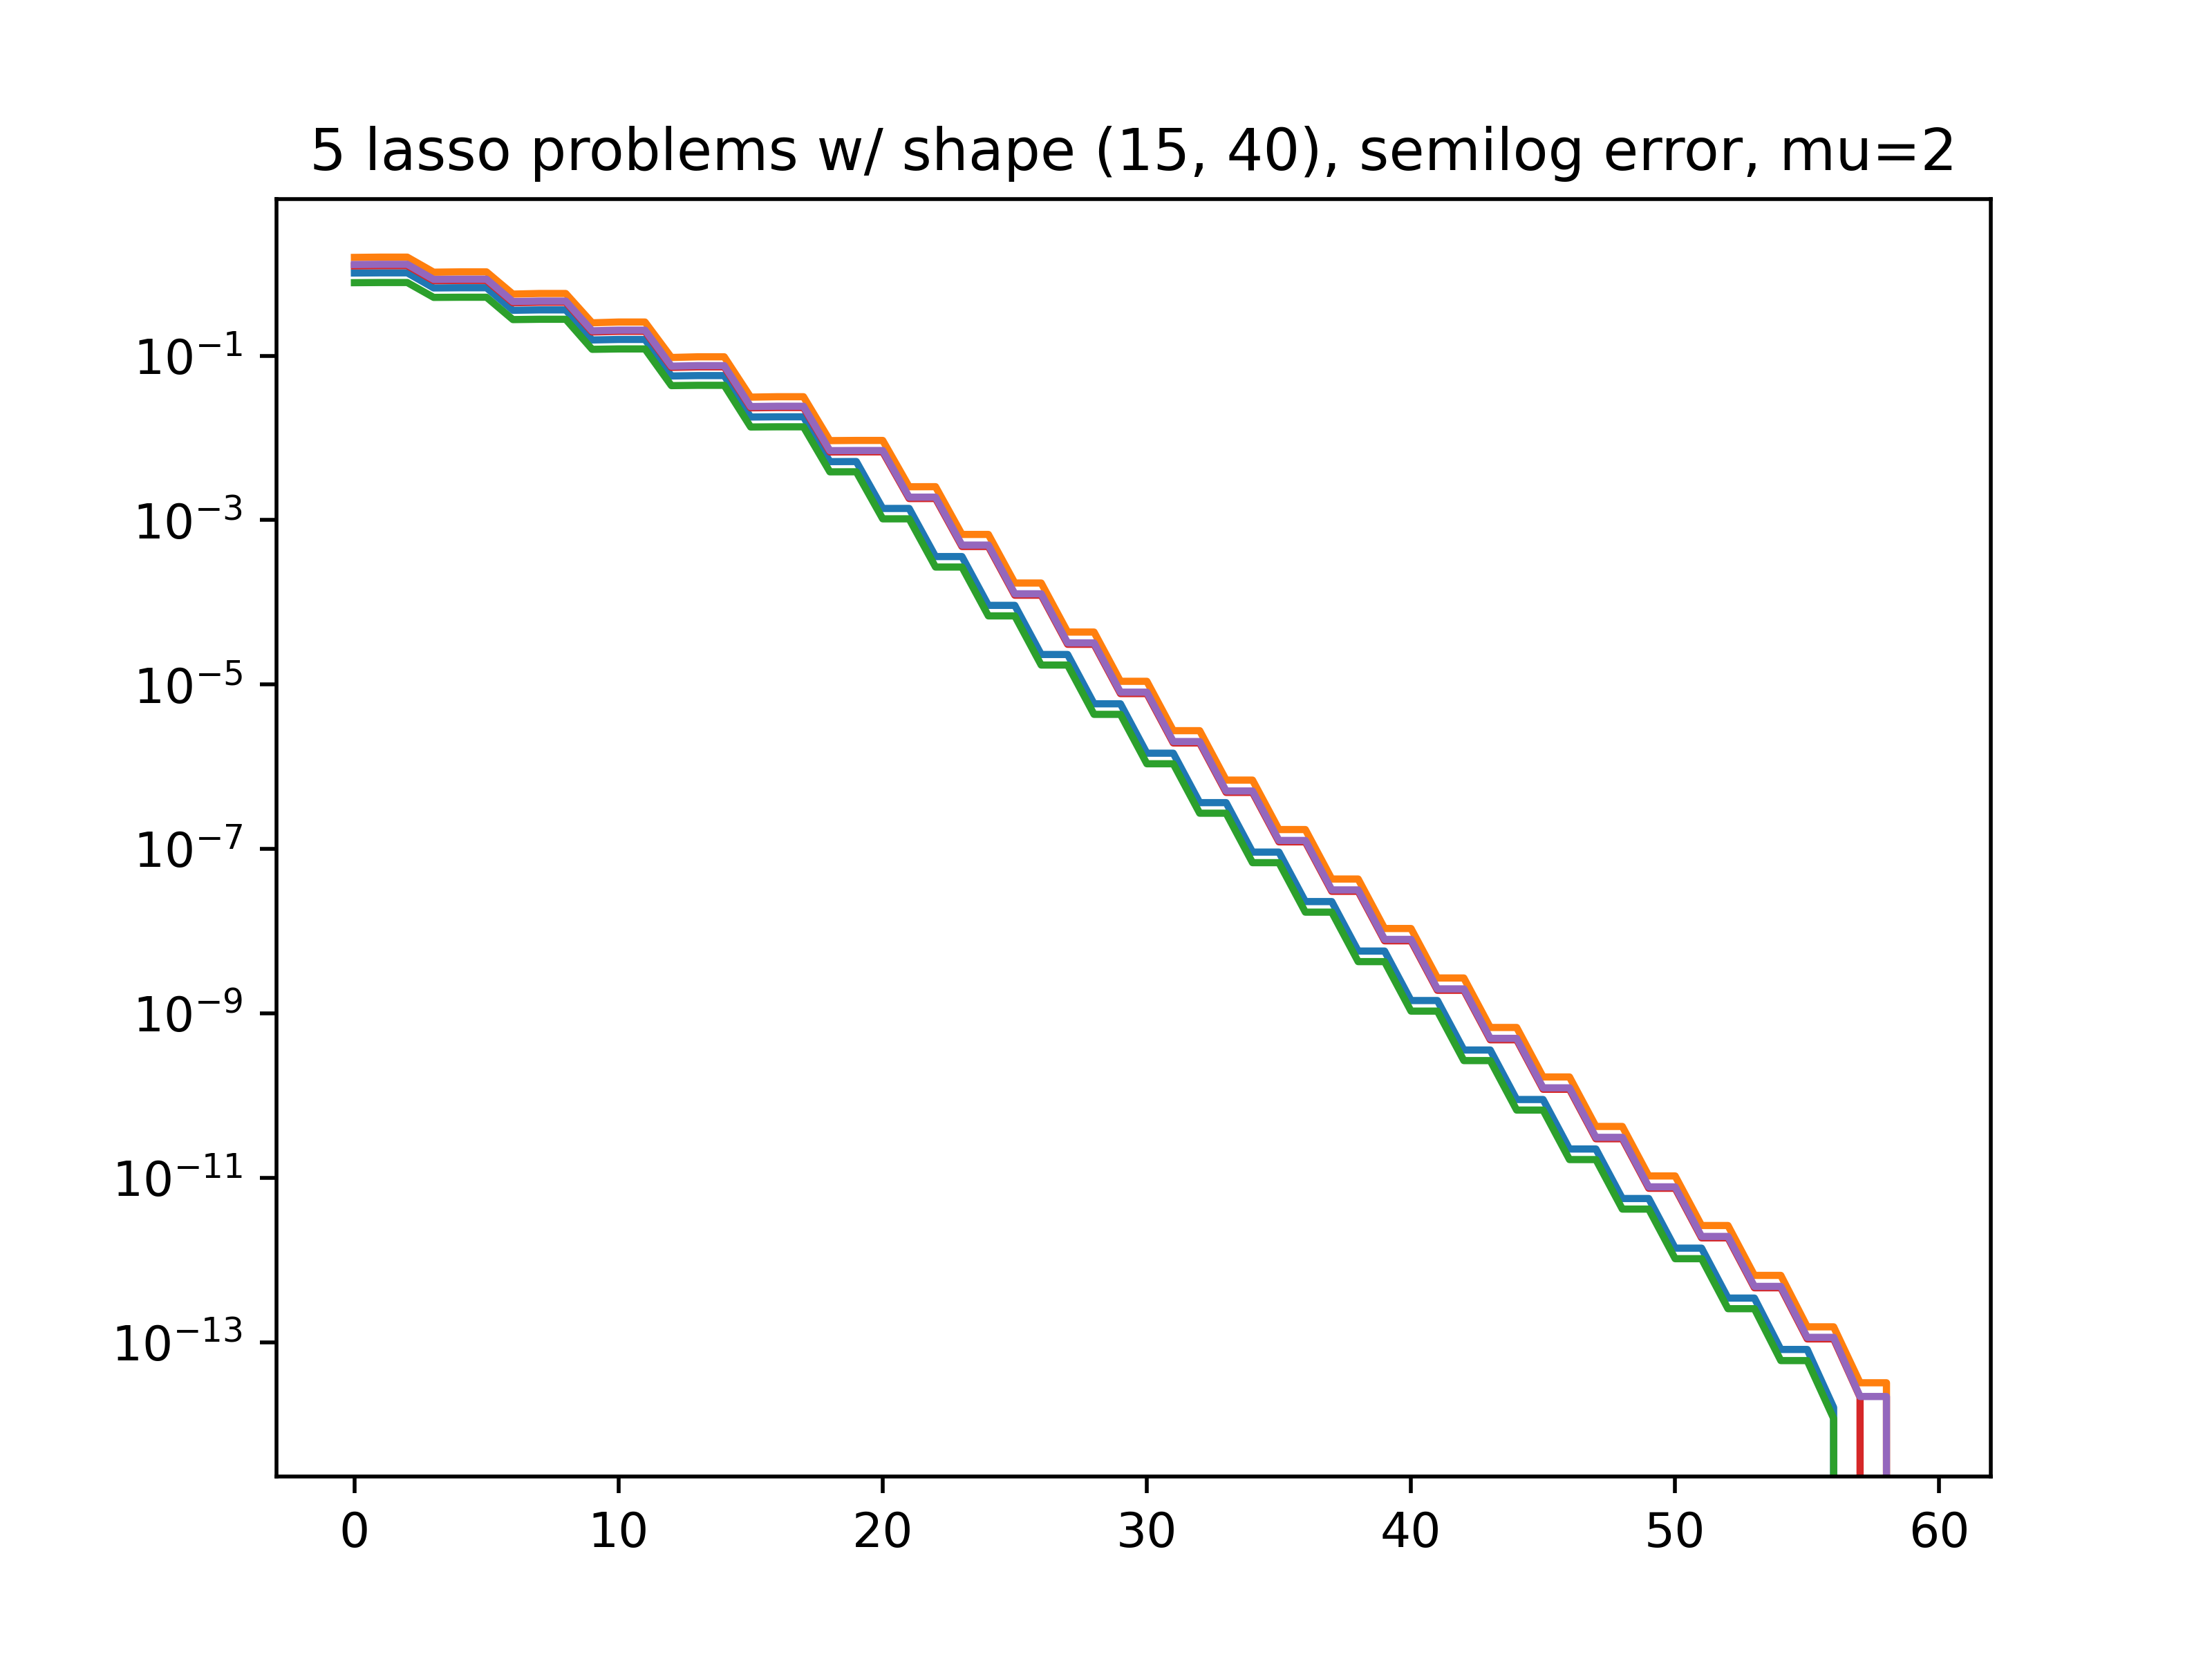
\includegraphics[width=.8\linewidth]{lasso_qp_2.png}
  \caption{1a}
  \label{fig:sfig1}
\end{subfigure}%
\begin{subfigure}{.5\textwidth}
  \centering
  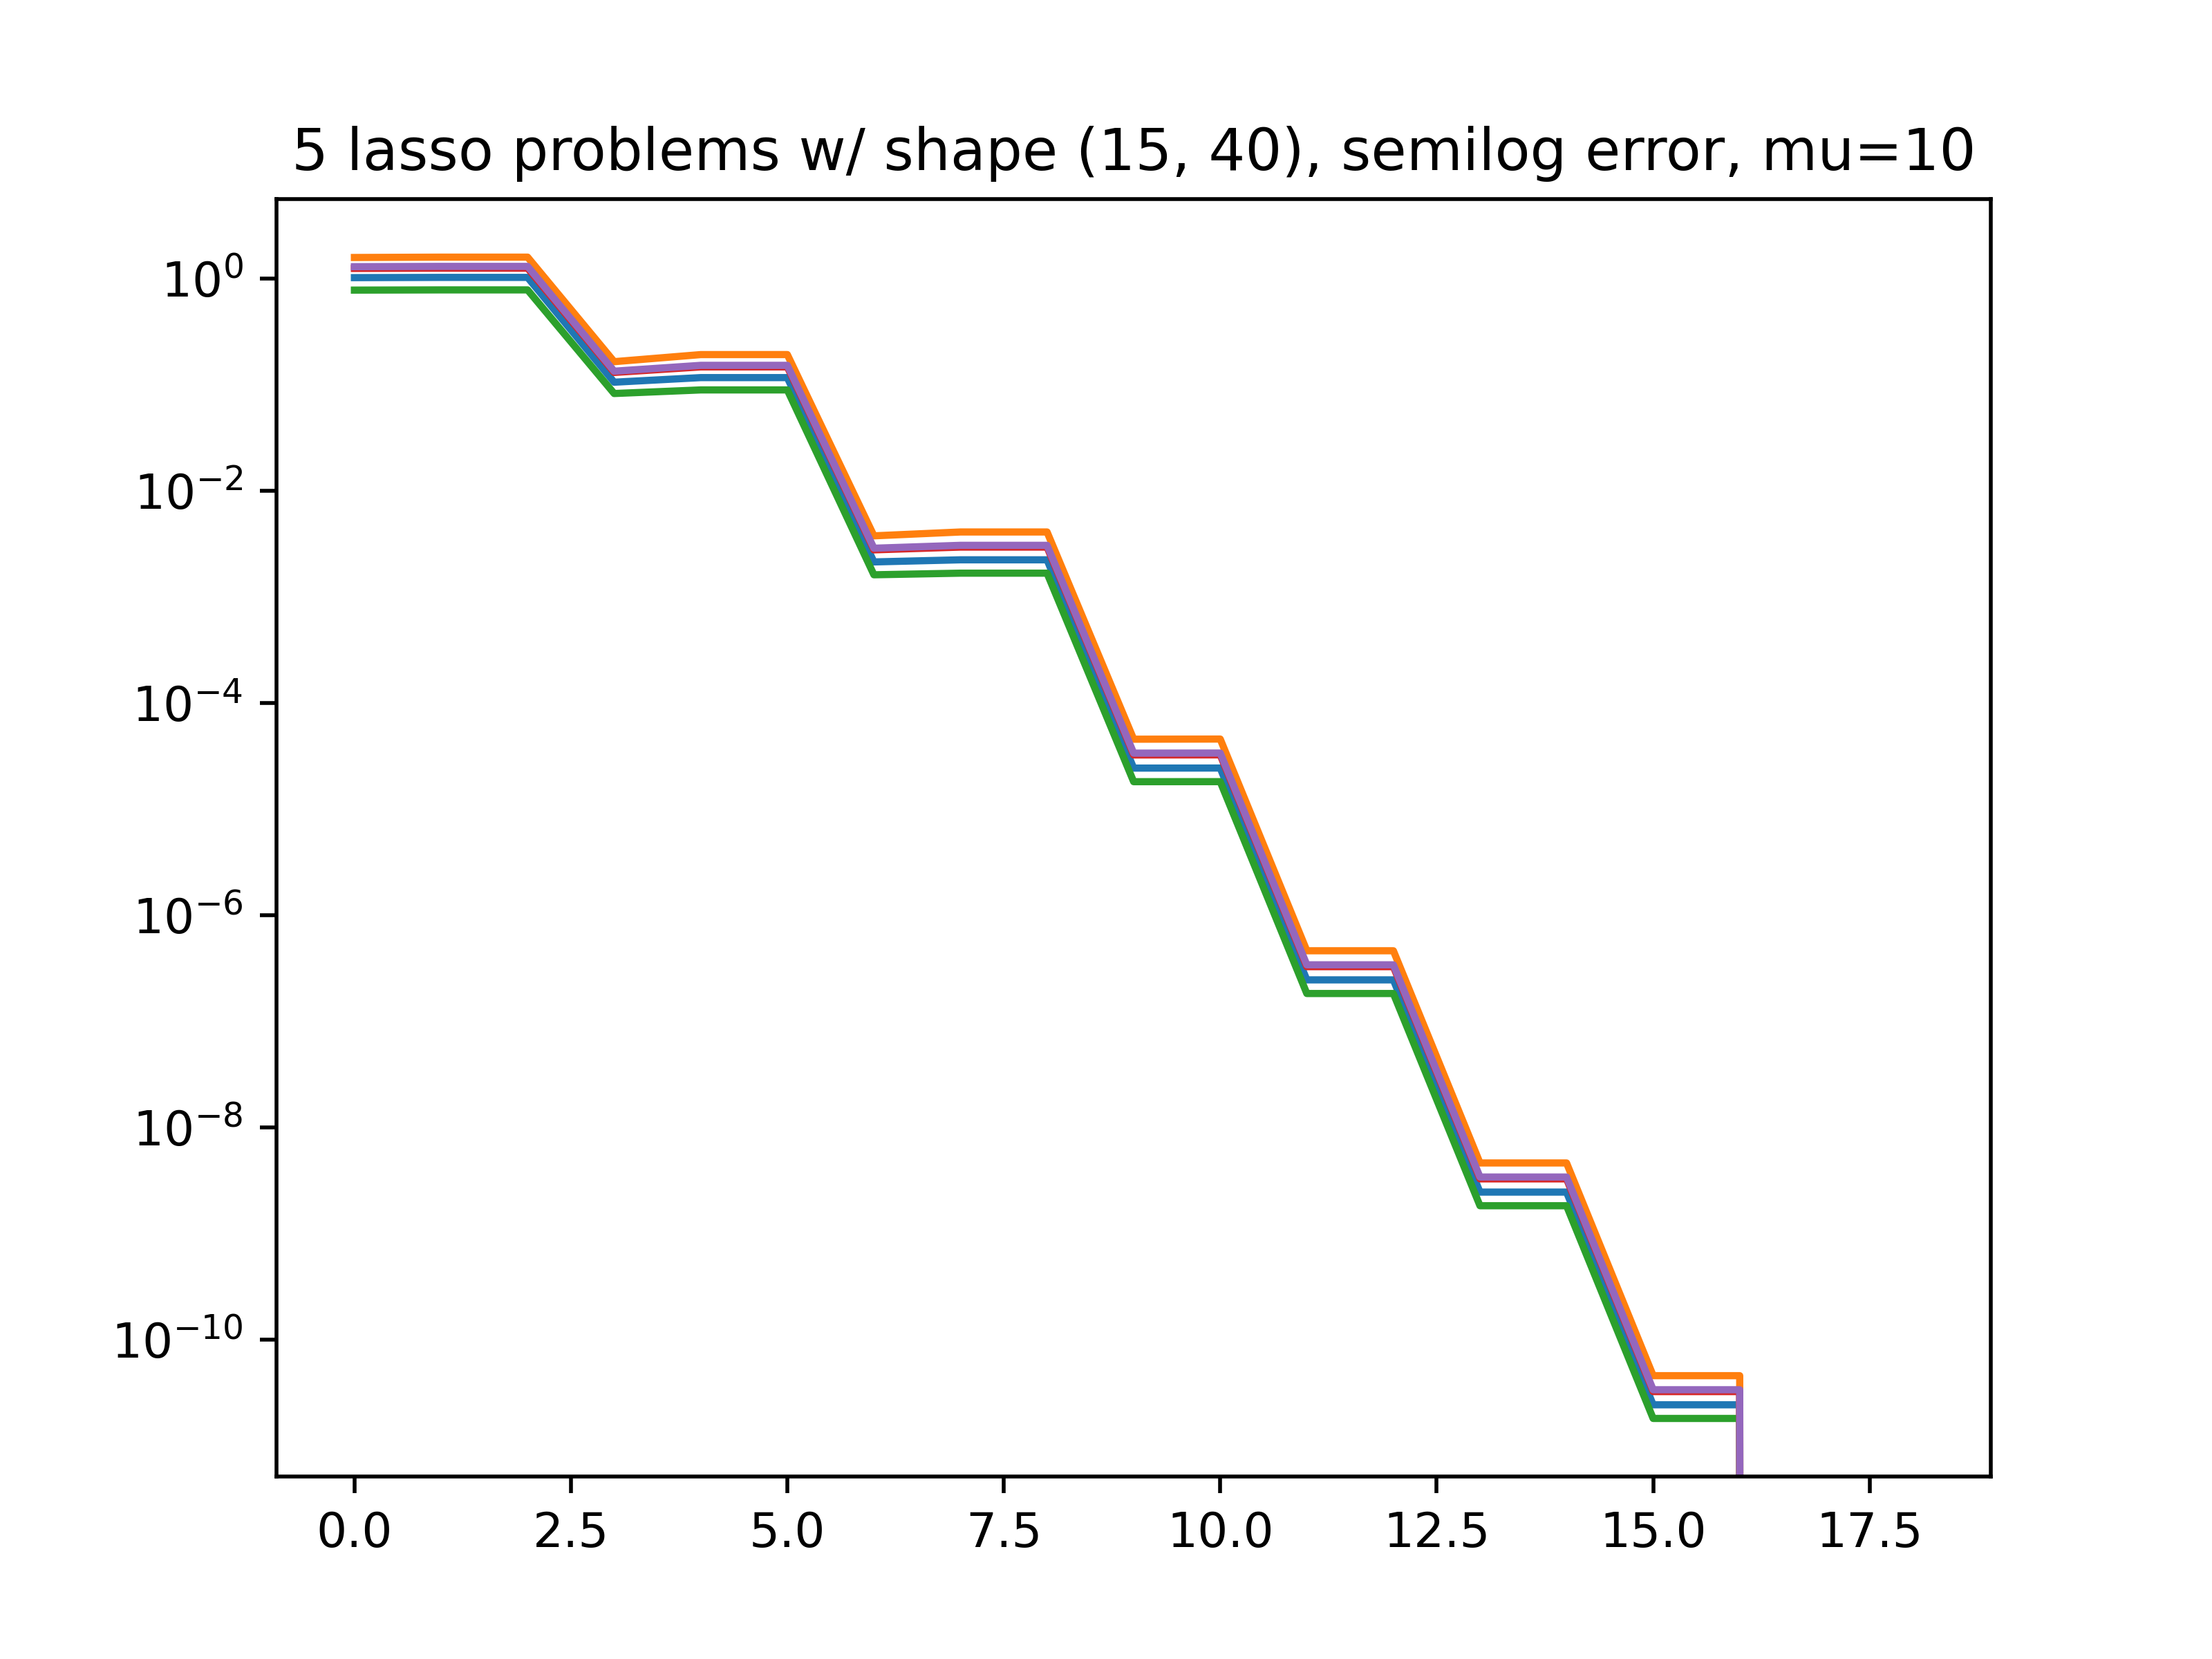
\includegraphics[width=.8\linewidth]{lasso_qp_10.png}
  \caption{1b}
  \label{fig:sfig2}
\end{subfigure}

\begin{subfigure}{.5\textwidth}
  \centering
  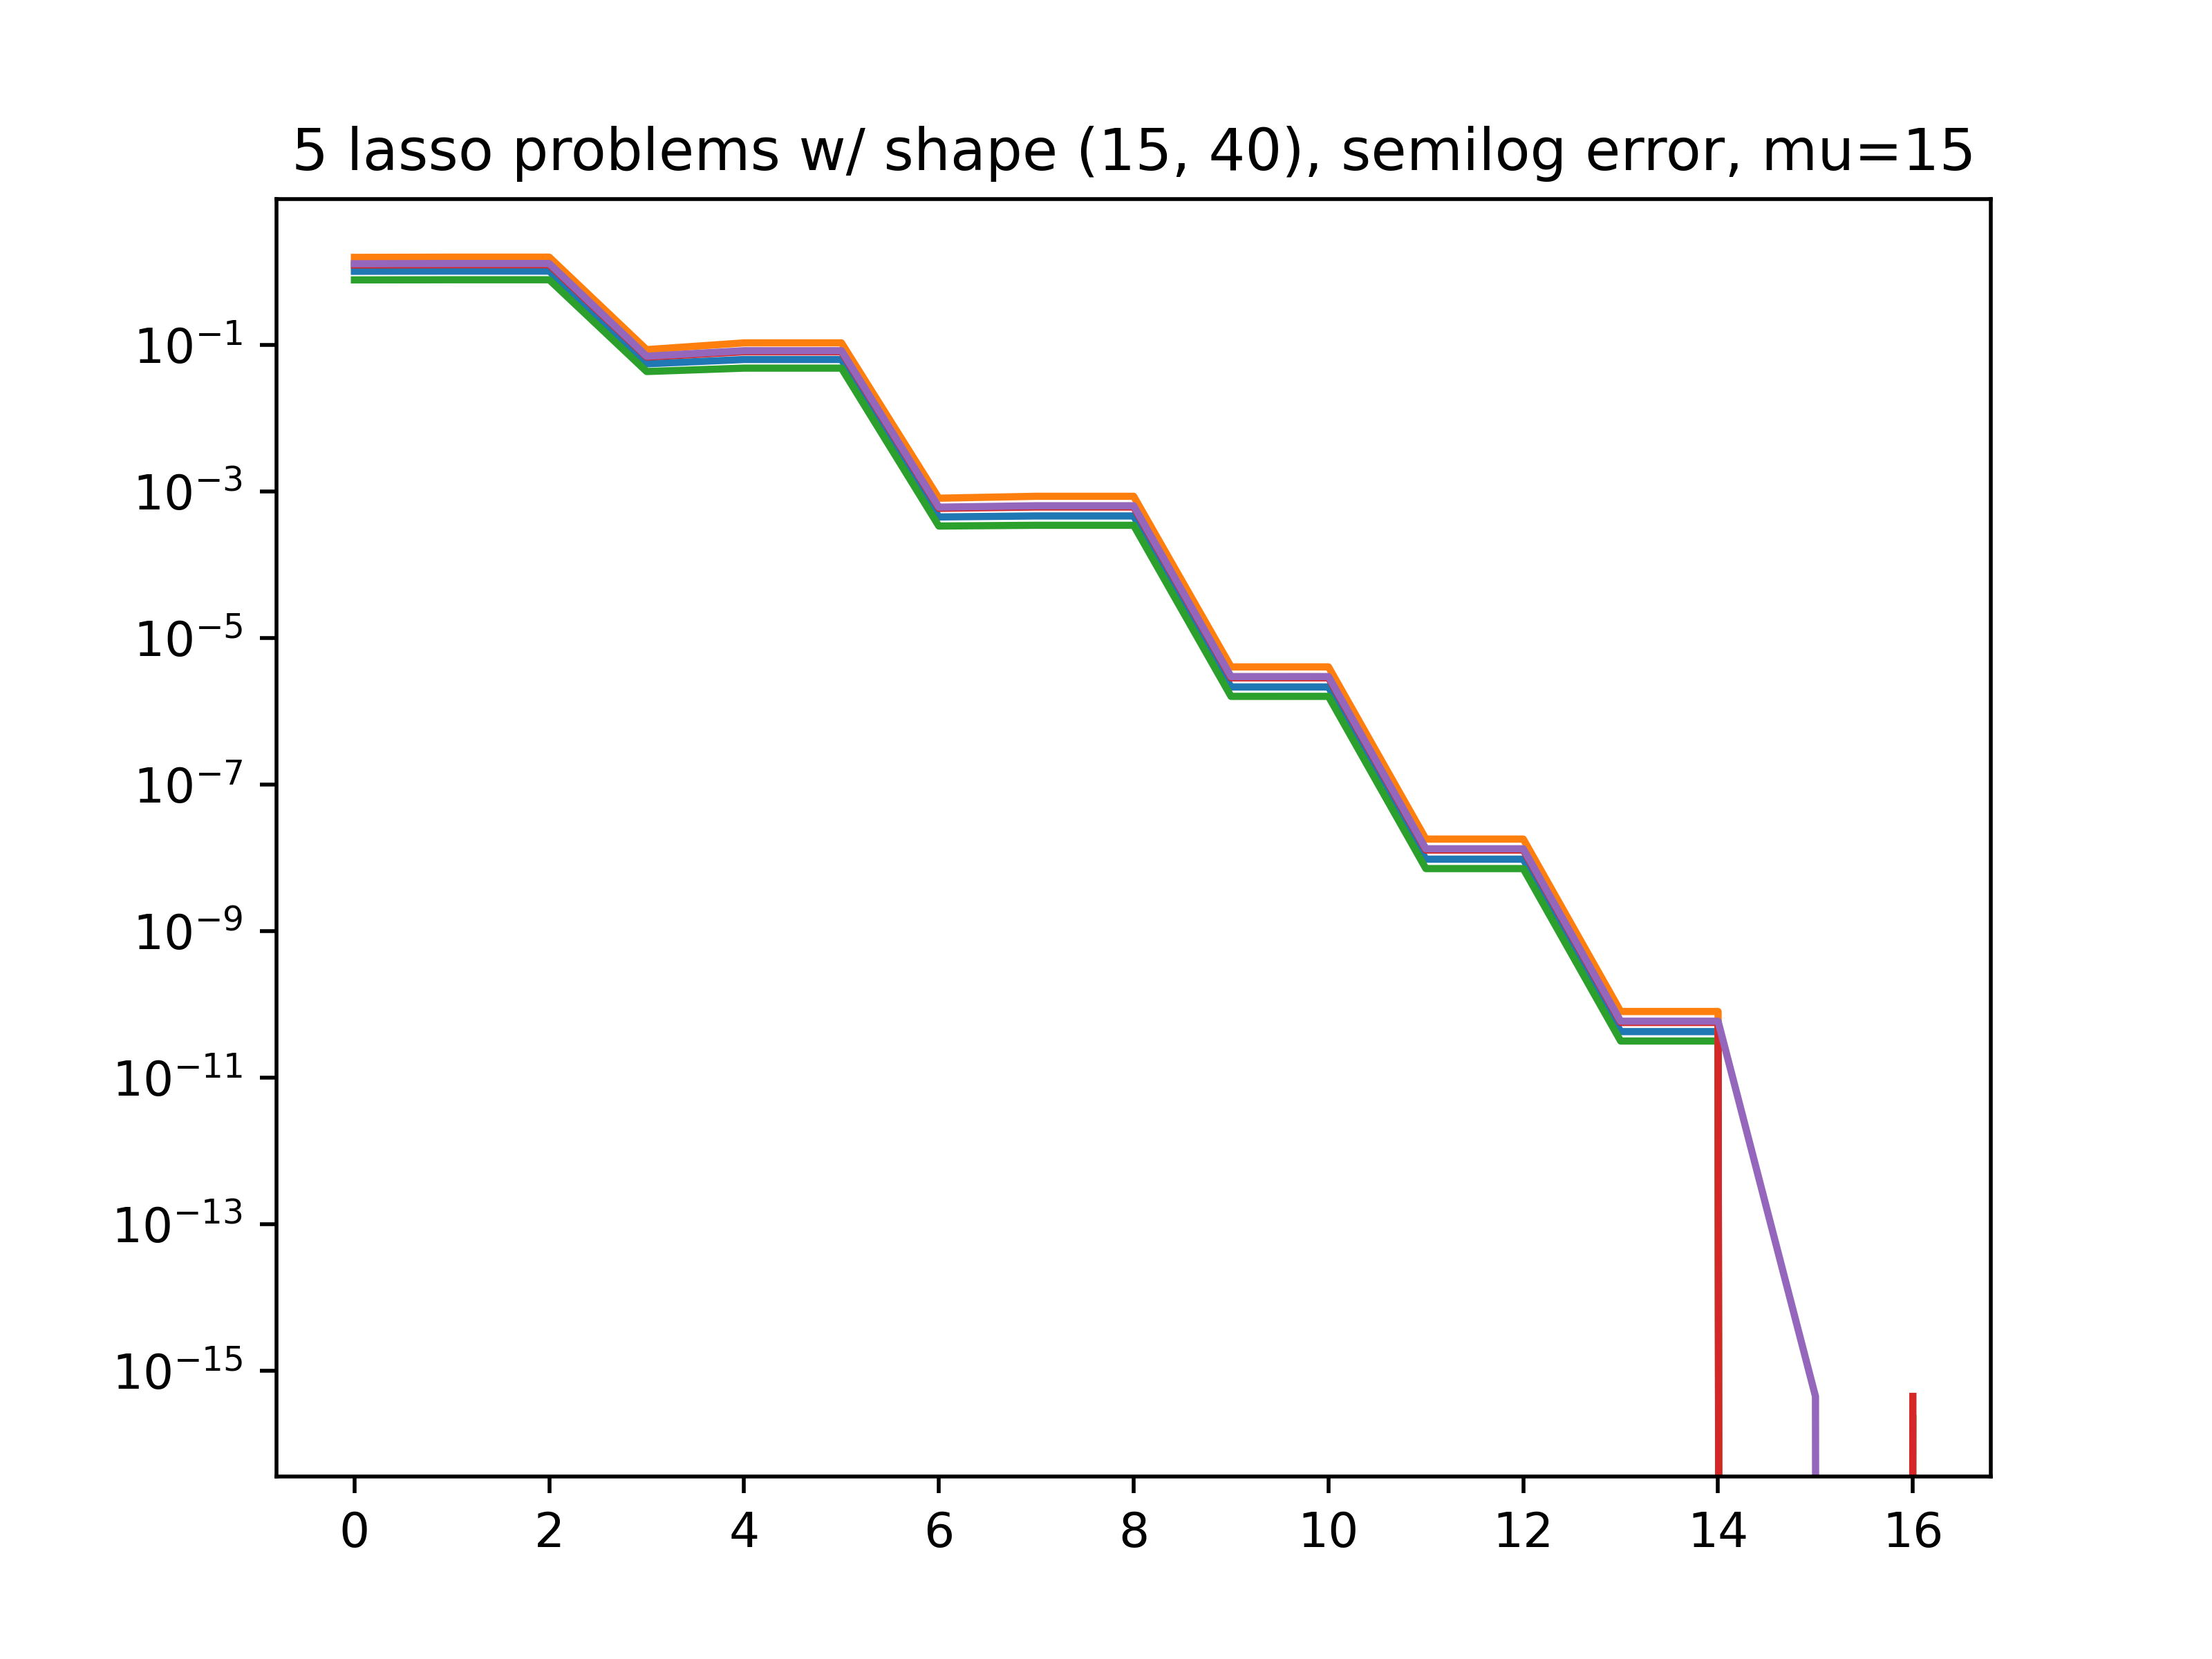
\includegraphics[width=.8\linewidth]{lasso_qp_15.png}
  \caption{1a}
  \label{fig:sfig1}
\end{subfigure}%
\begin{subfigure}{.5\textwidth}
  \centering
  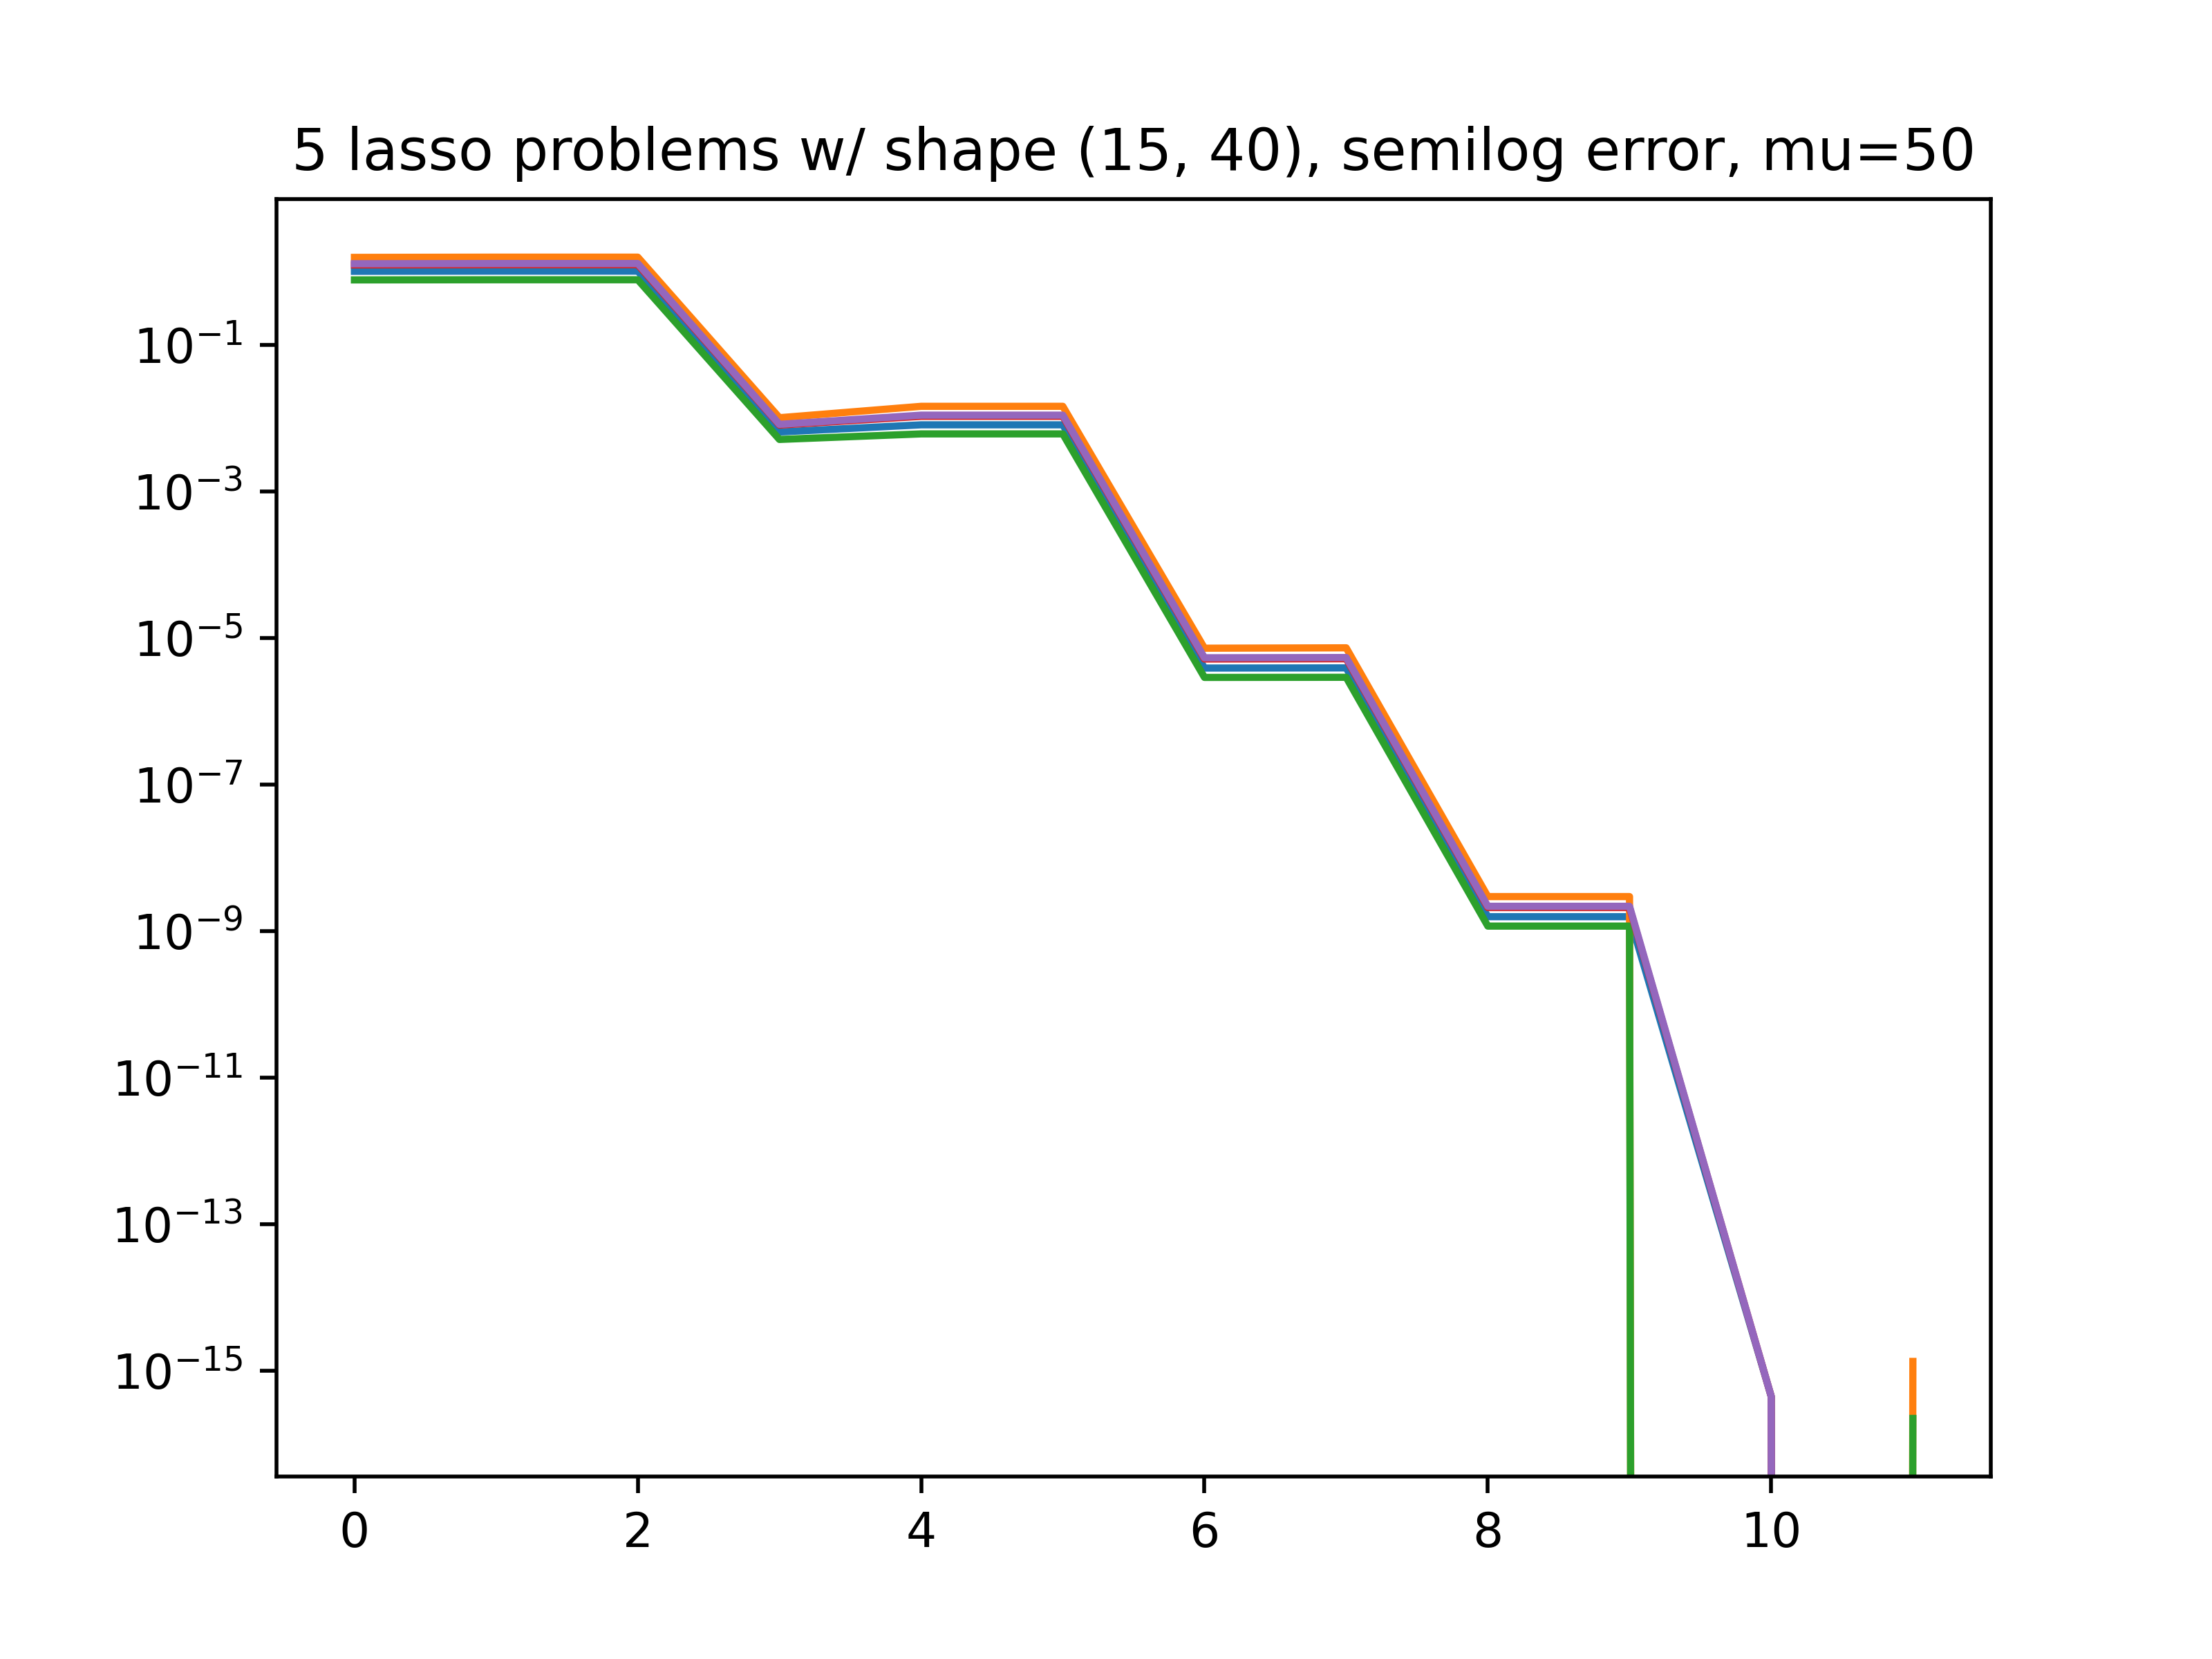
\includegraphics[width=.8\linewidth]{lasso_qp_50.png}
  \caption{1b}
  \label{fig:sfig2}
\end{subfigure}

\begin{subfigure}{.5\textwidth}
  \centering
  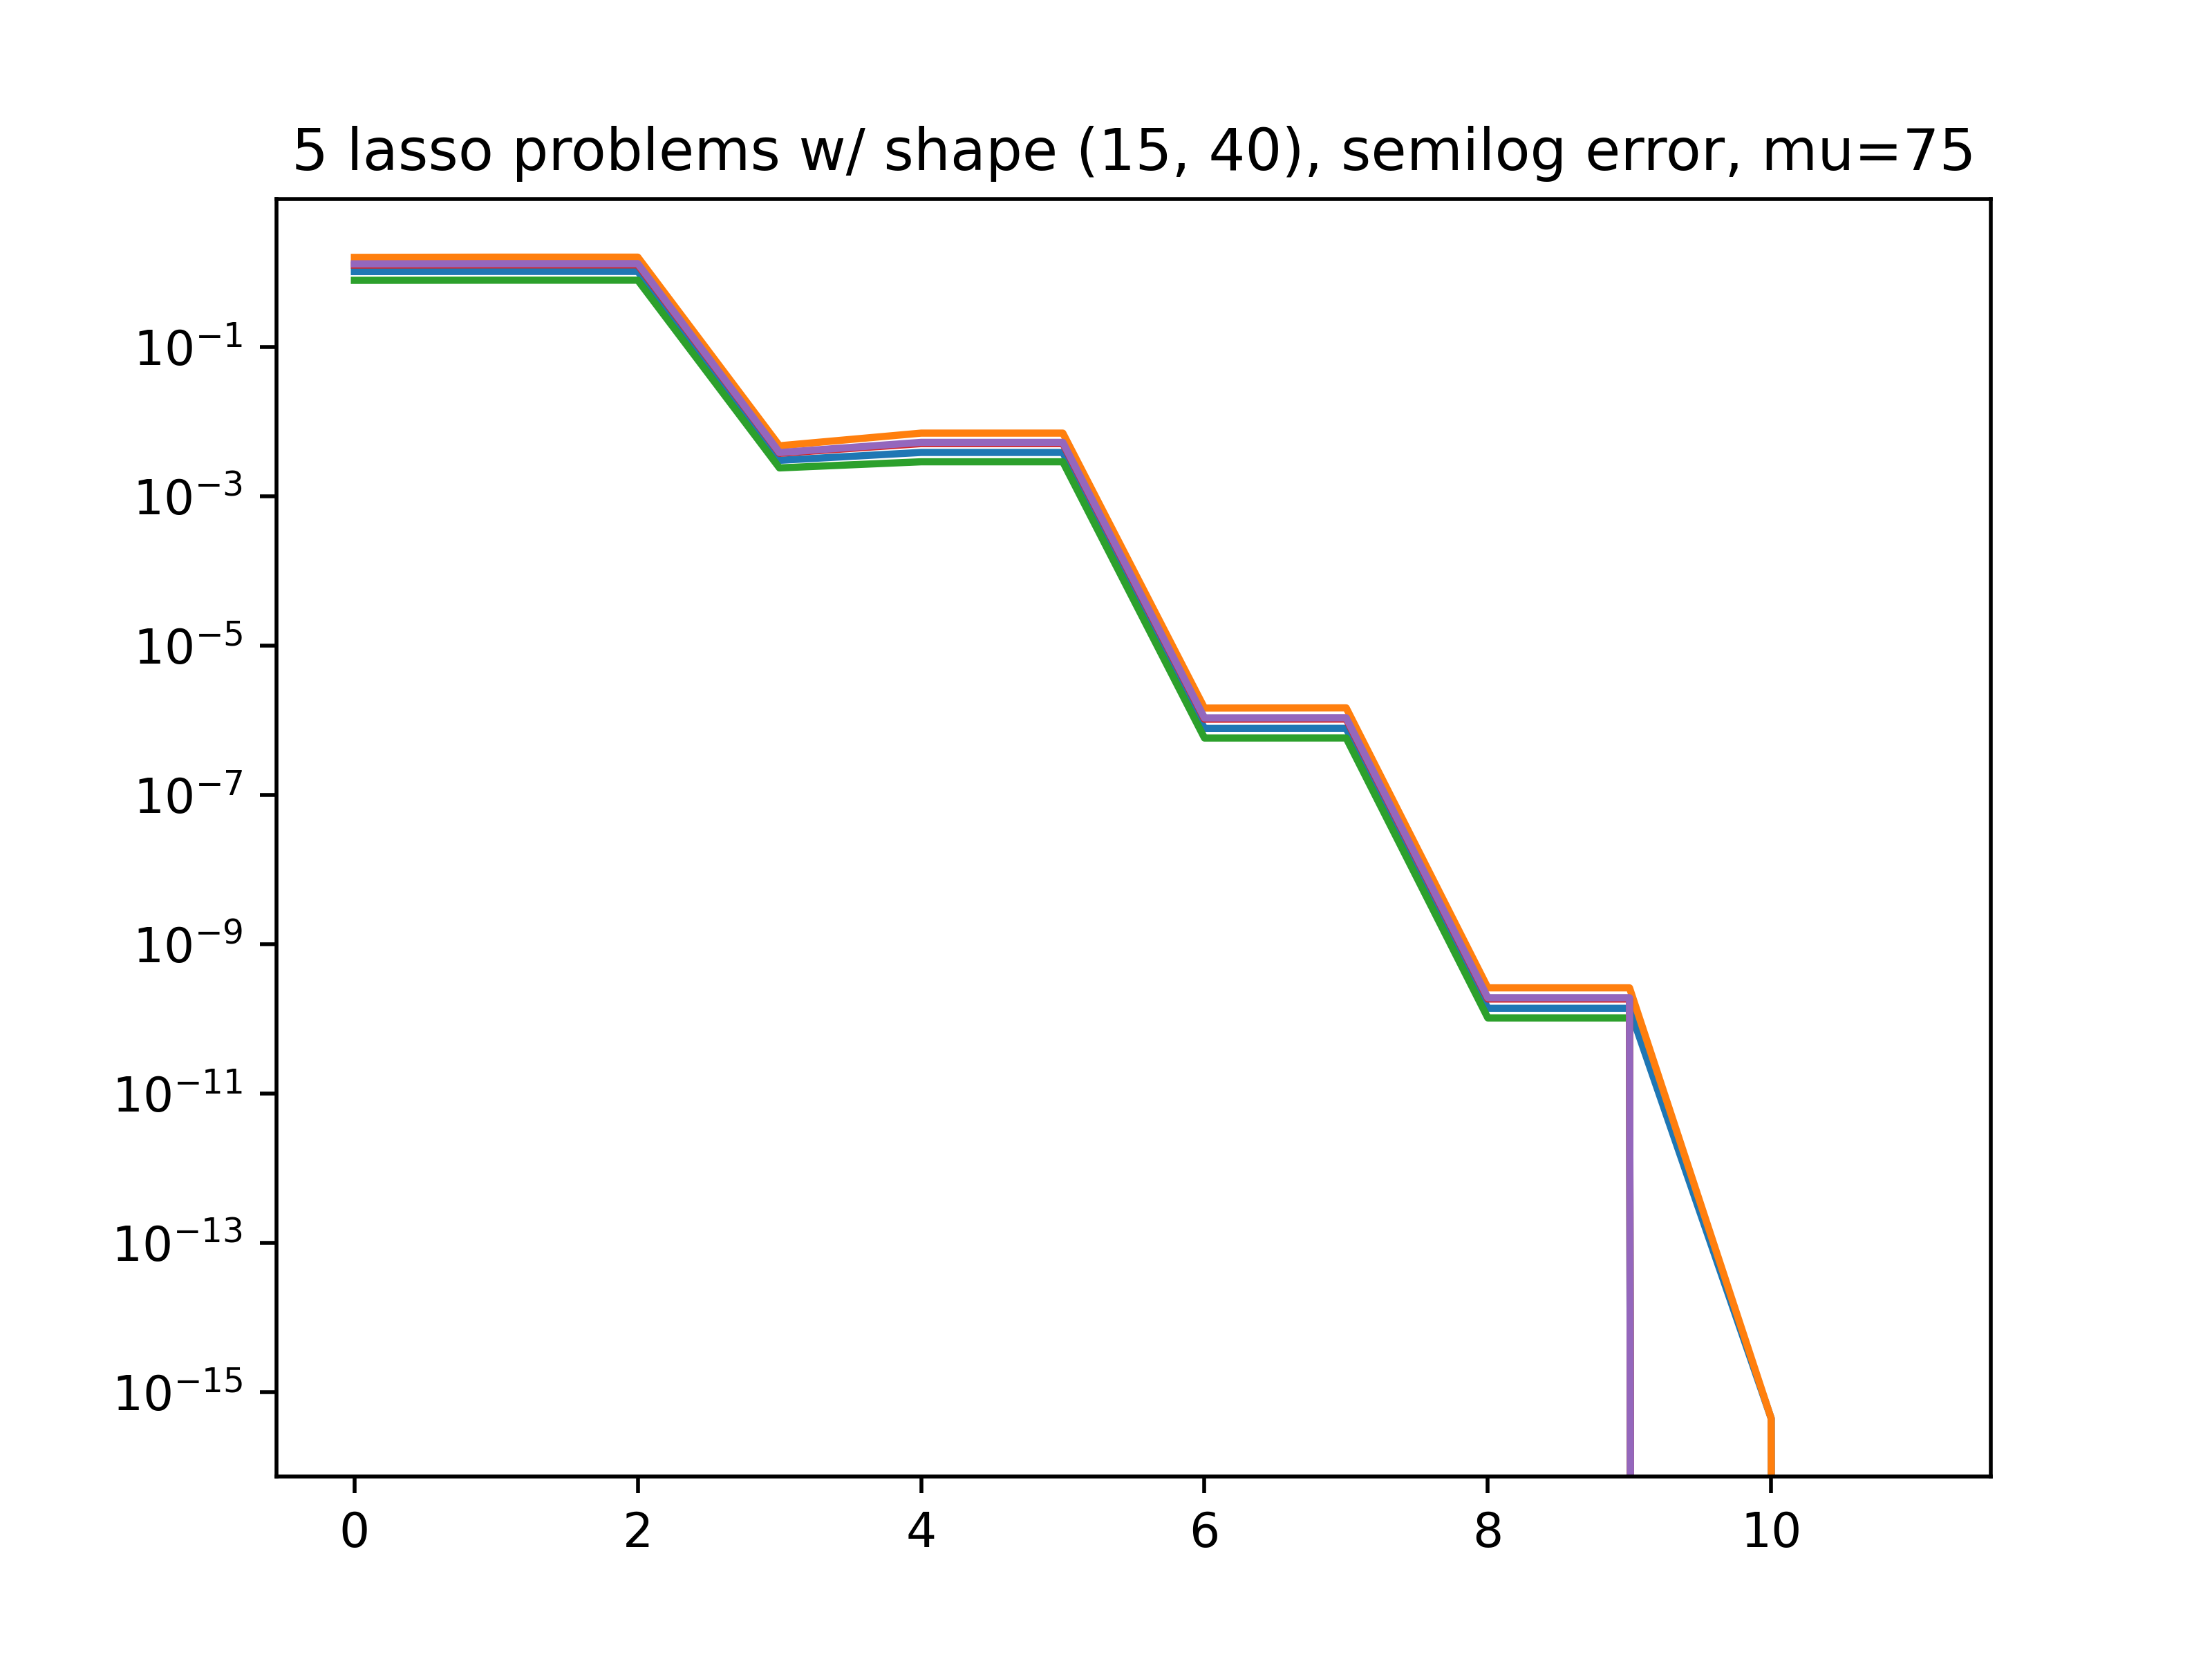
\includegraphics[width=.8\linewidth]{lasso_qp_75.png}
  \caption{1a}
  \label{fig:sfig1}
\end{subfigure}%
\begin{subfigure}{.5\textwidth}
  \centering
  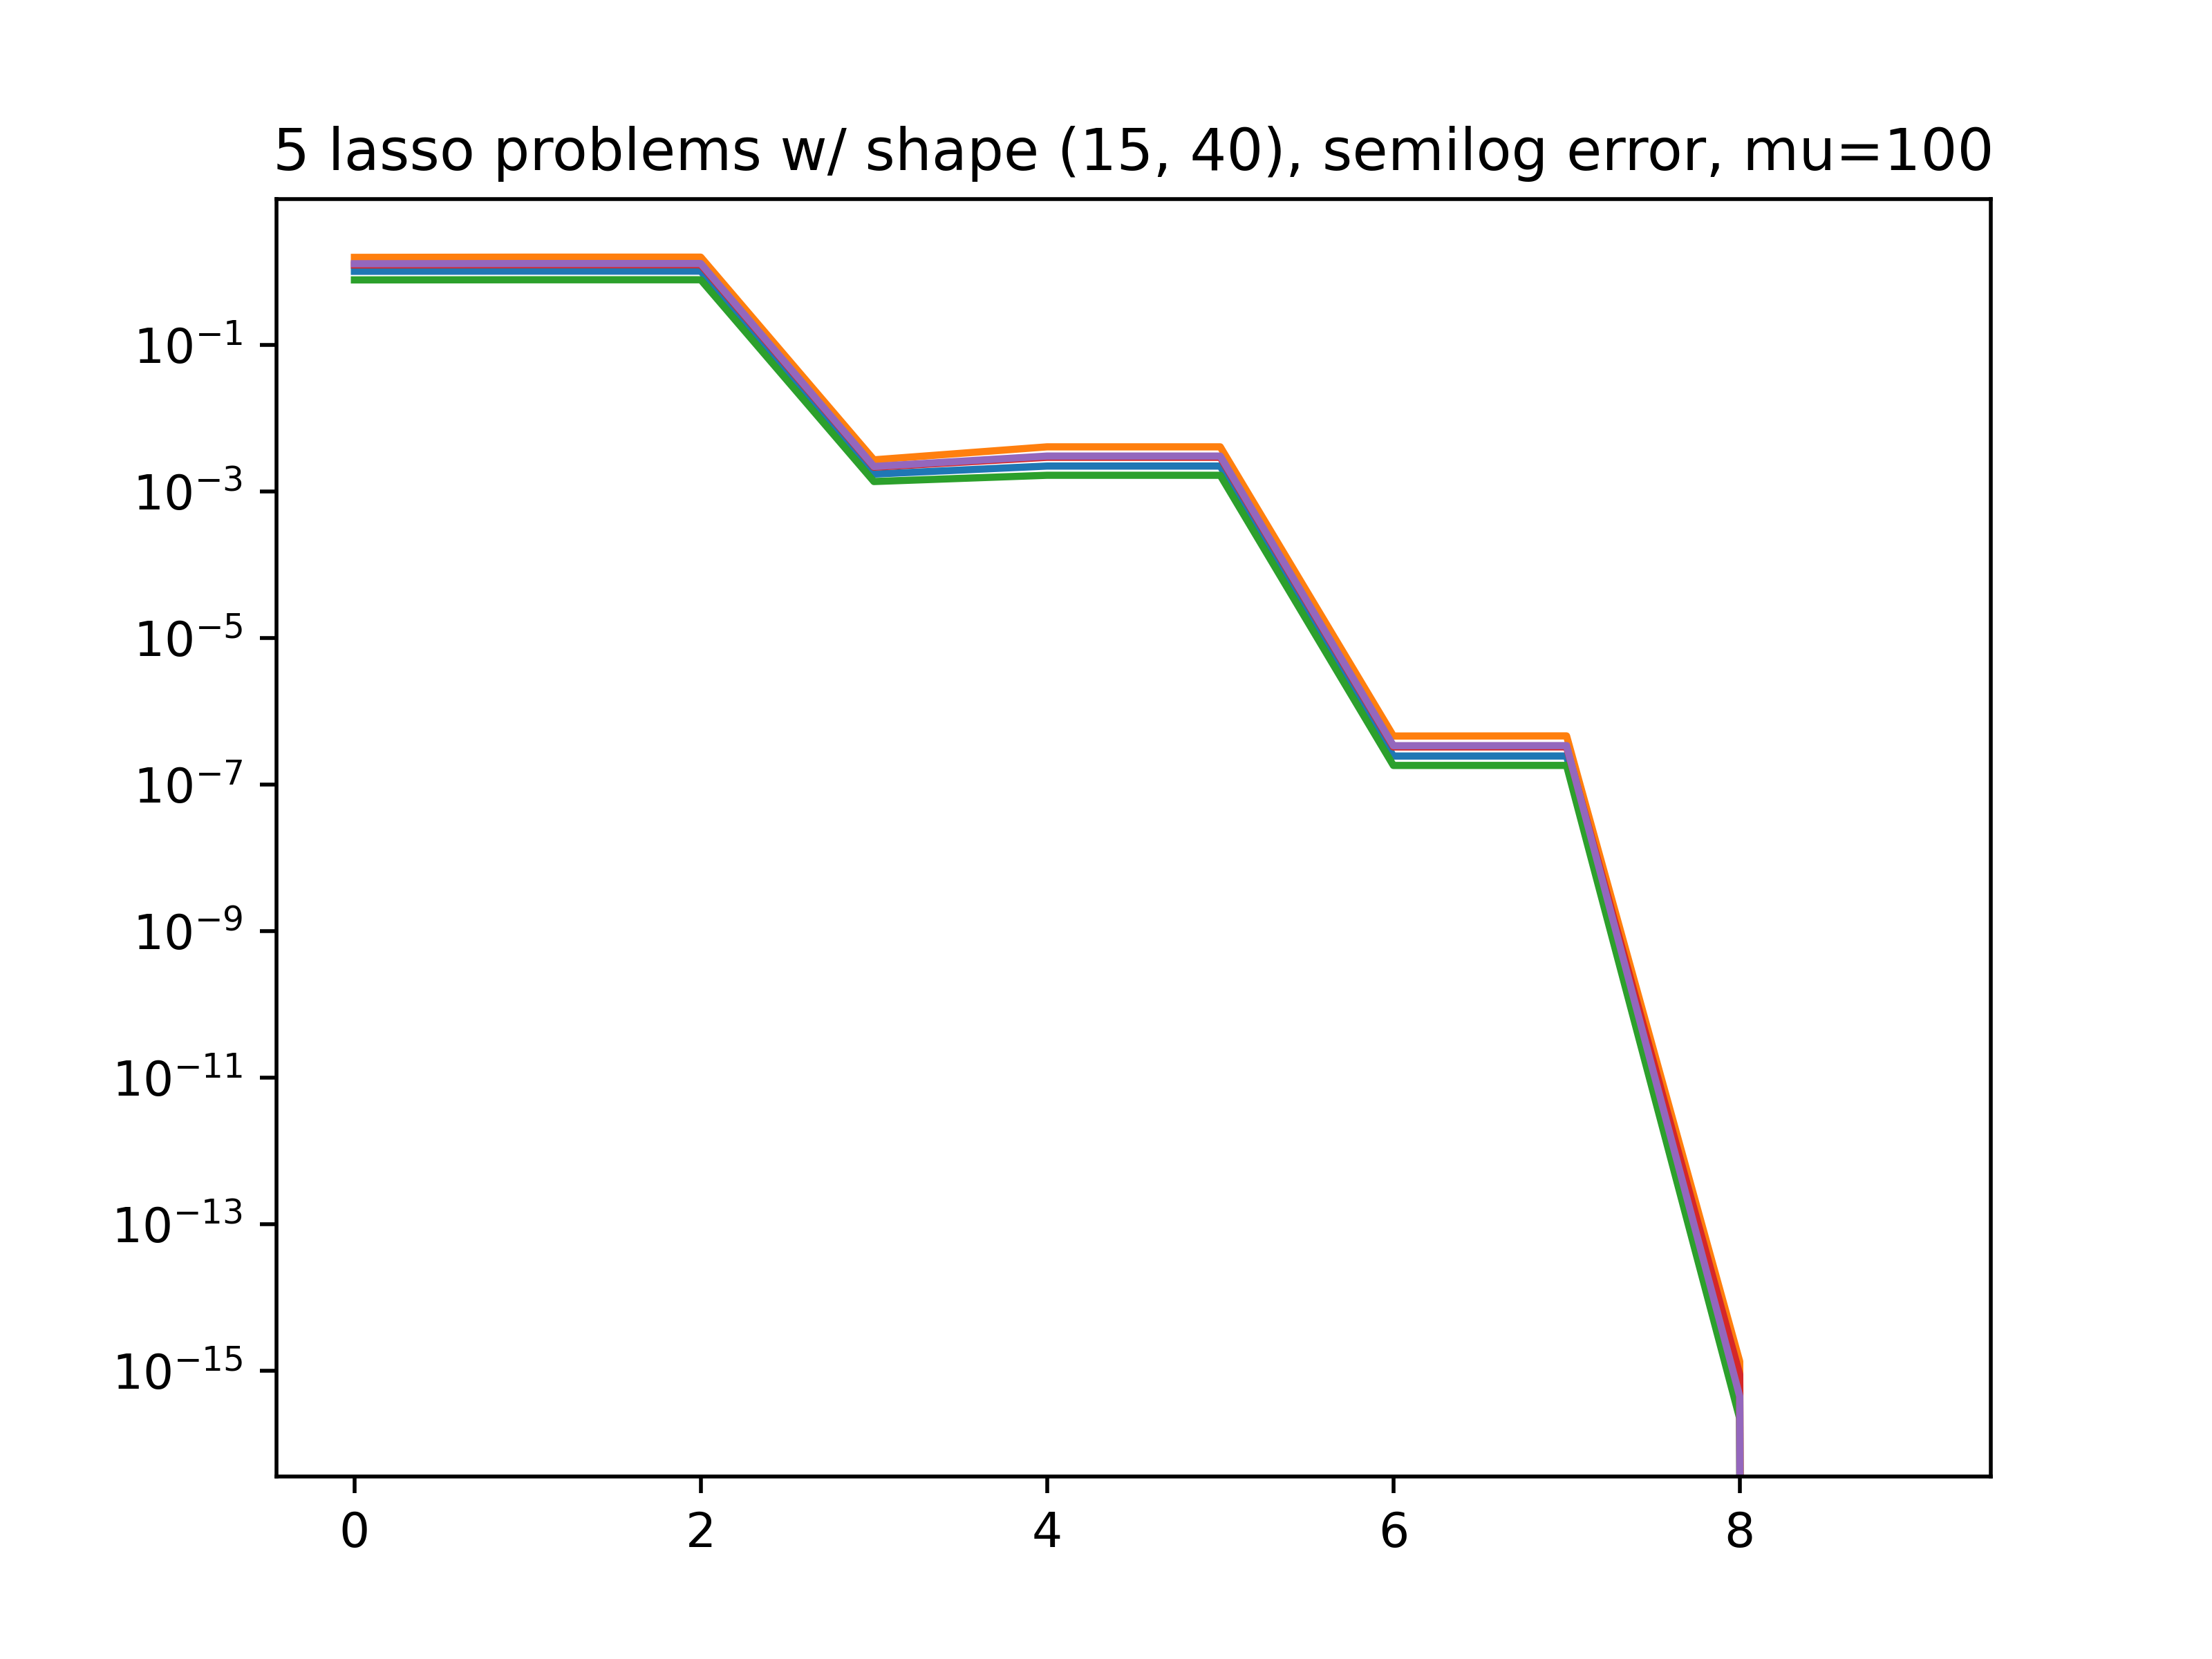
\includegraphics[width=.8\linewidth]{lasso_qp_100.png}
  \caption{1b}
  \label{fig:sfig2}
\end{subfigure}

\begin{subfigure}{.5\textwidth}
  \centering
  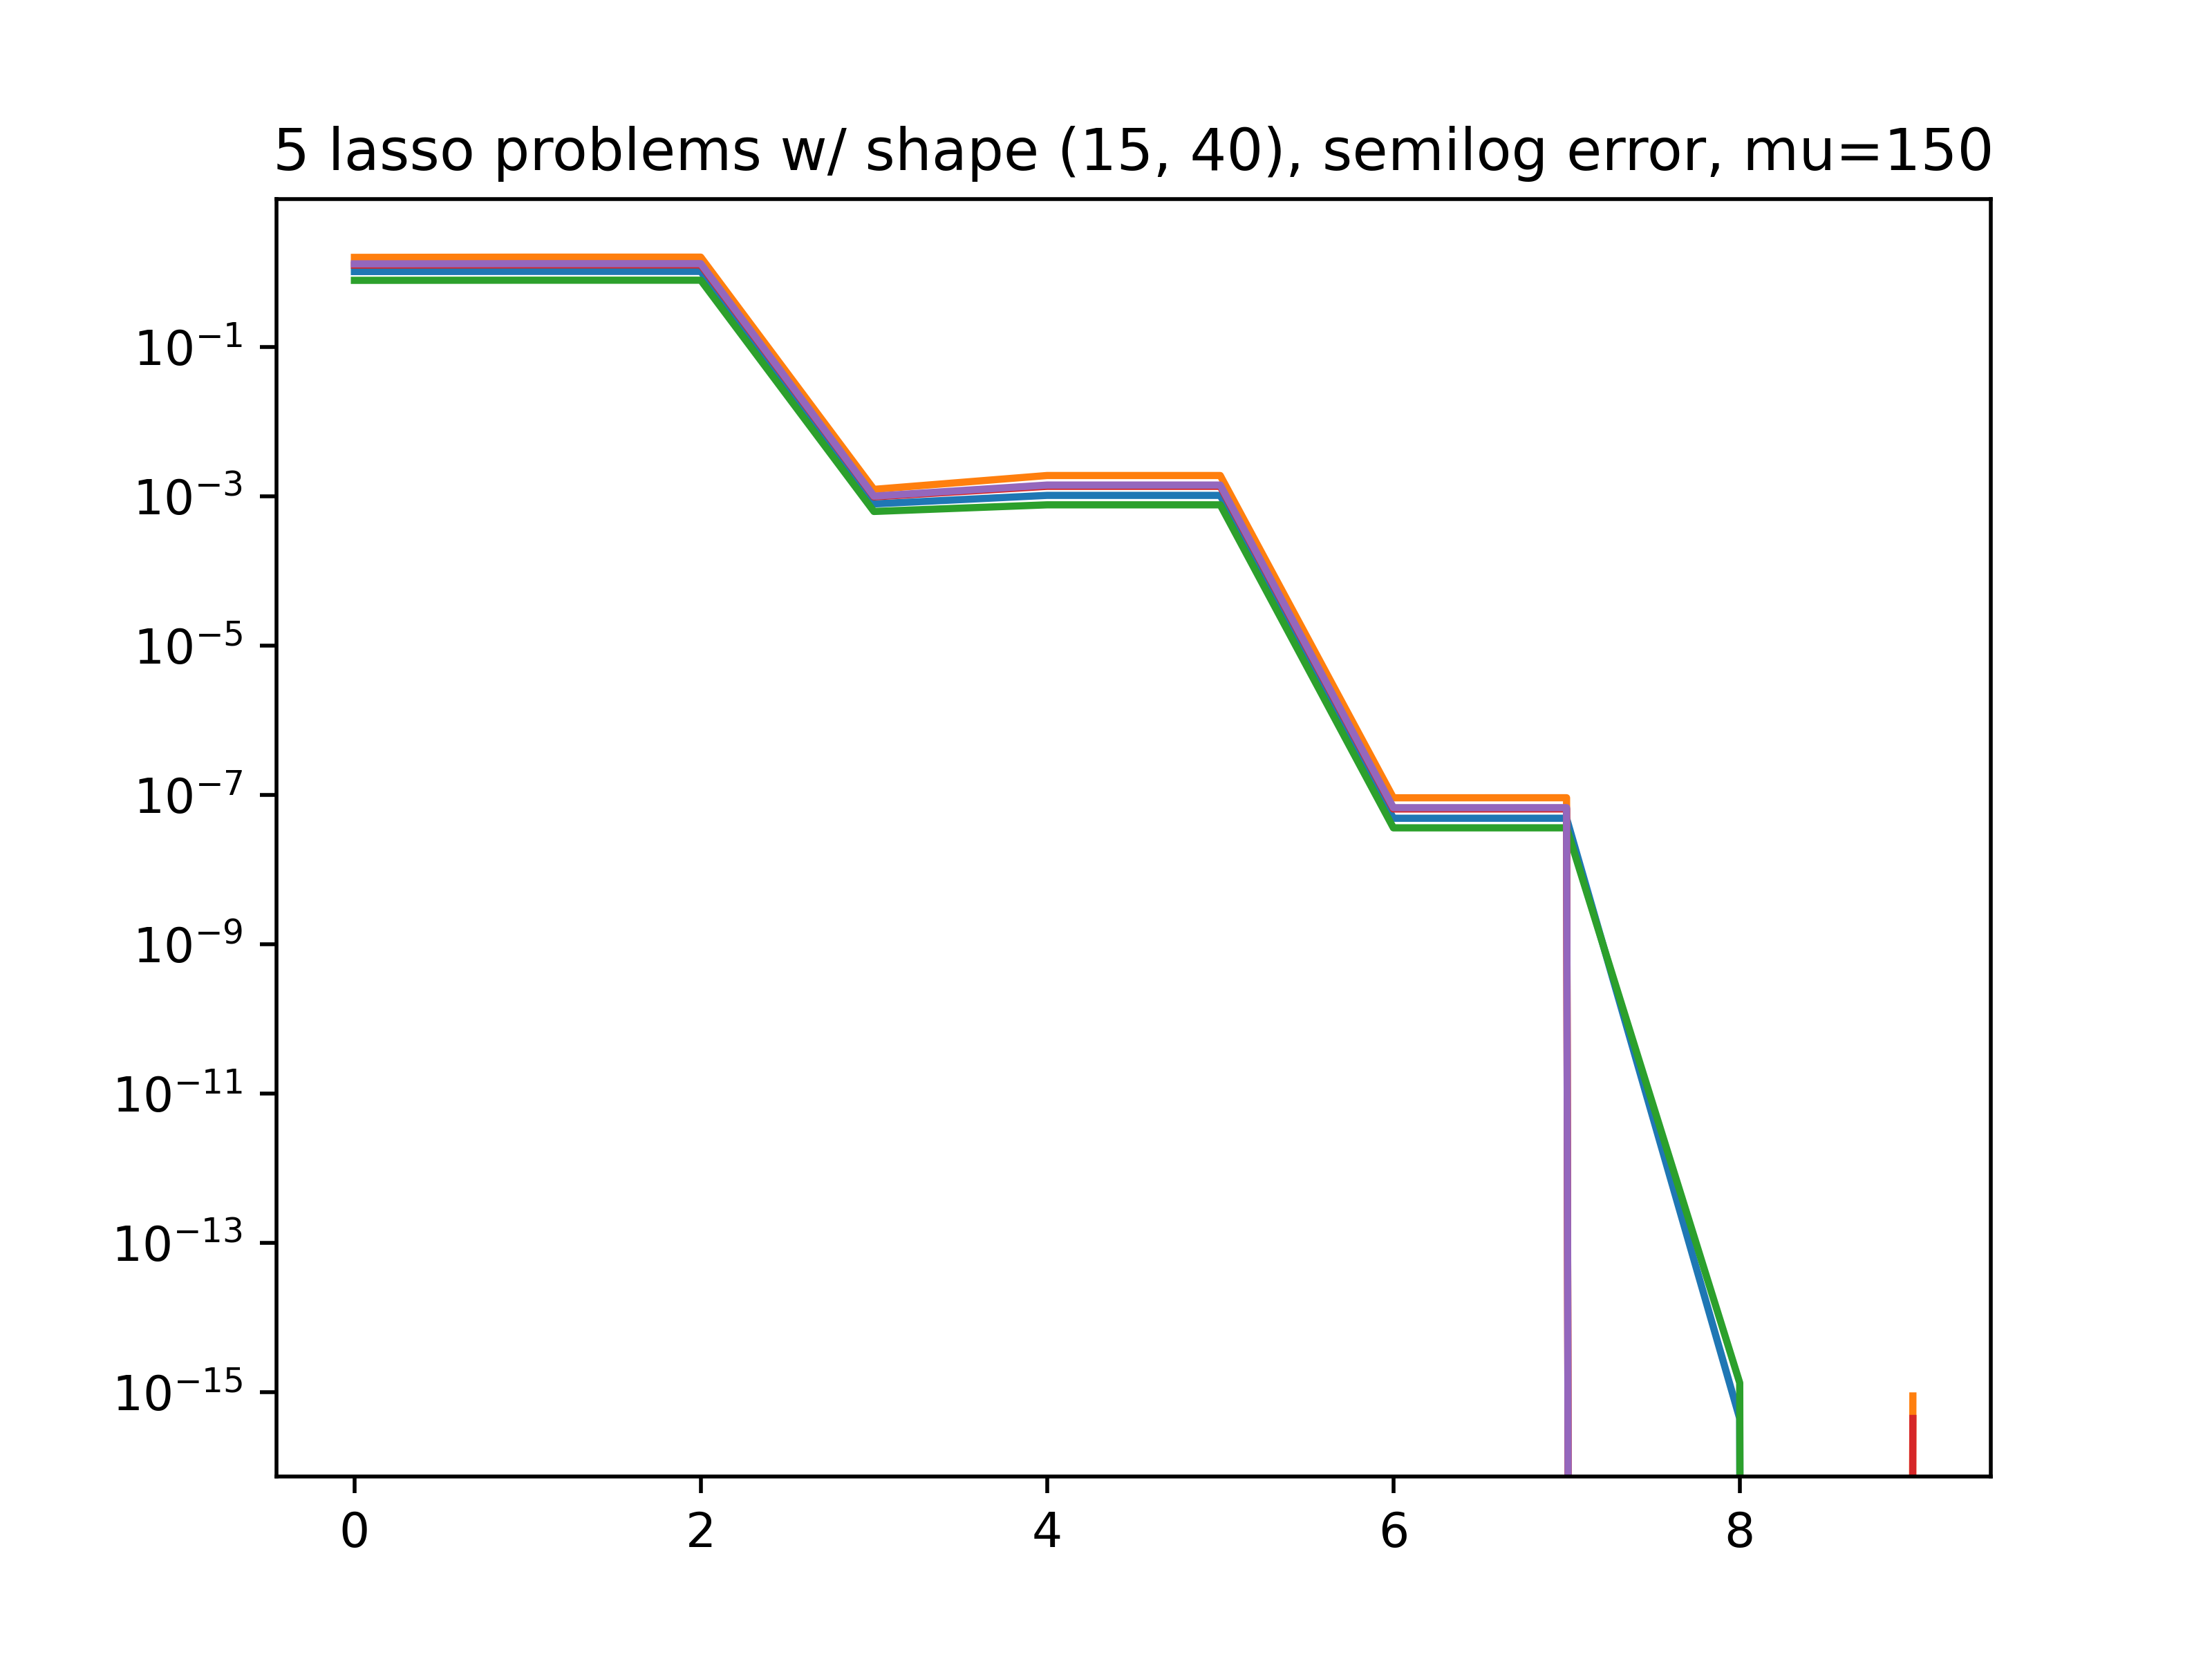
\includegraphics[width=.8\linewidth]{lasso_qp_150.png}
  \caption{1a}
  \label{fig:sfig1}
\end{subfigure}%
\begin{subfigure}{.5\textwidth}
  \centering
  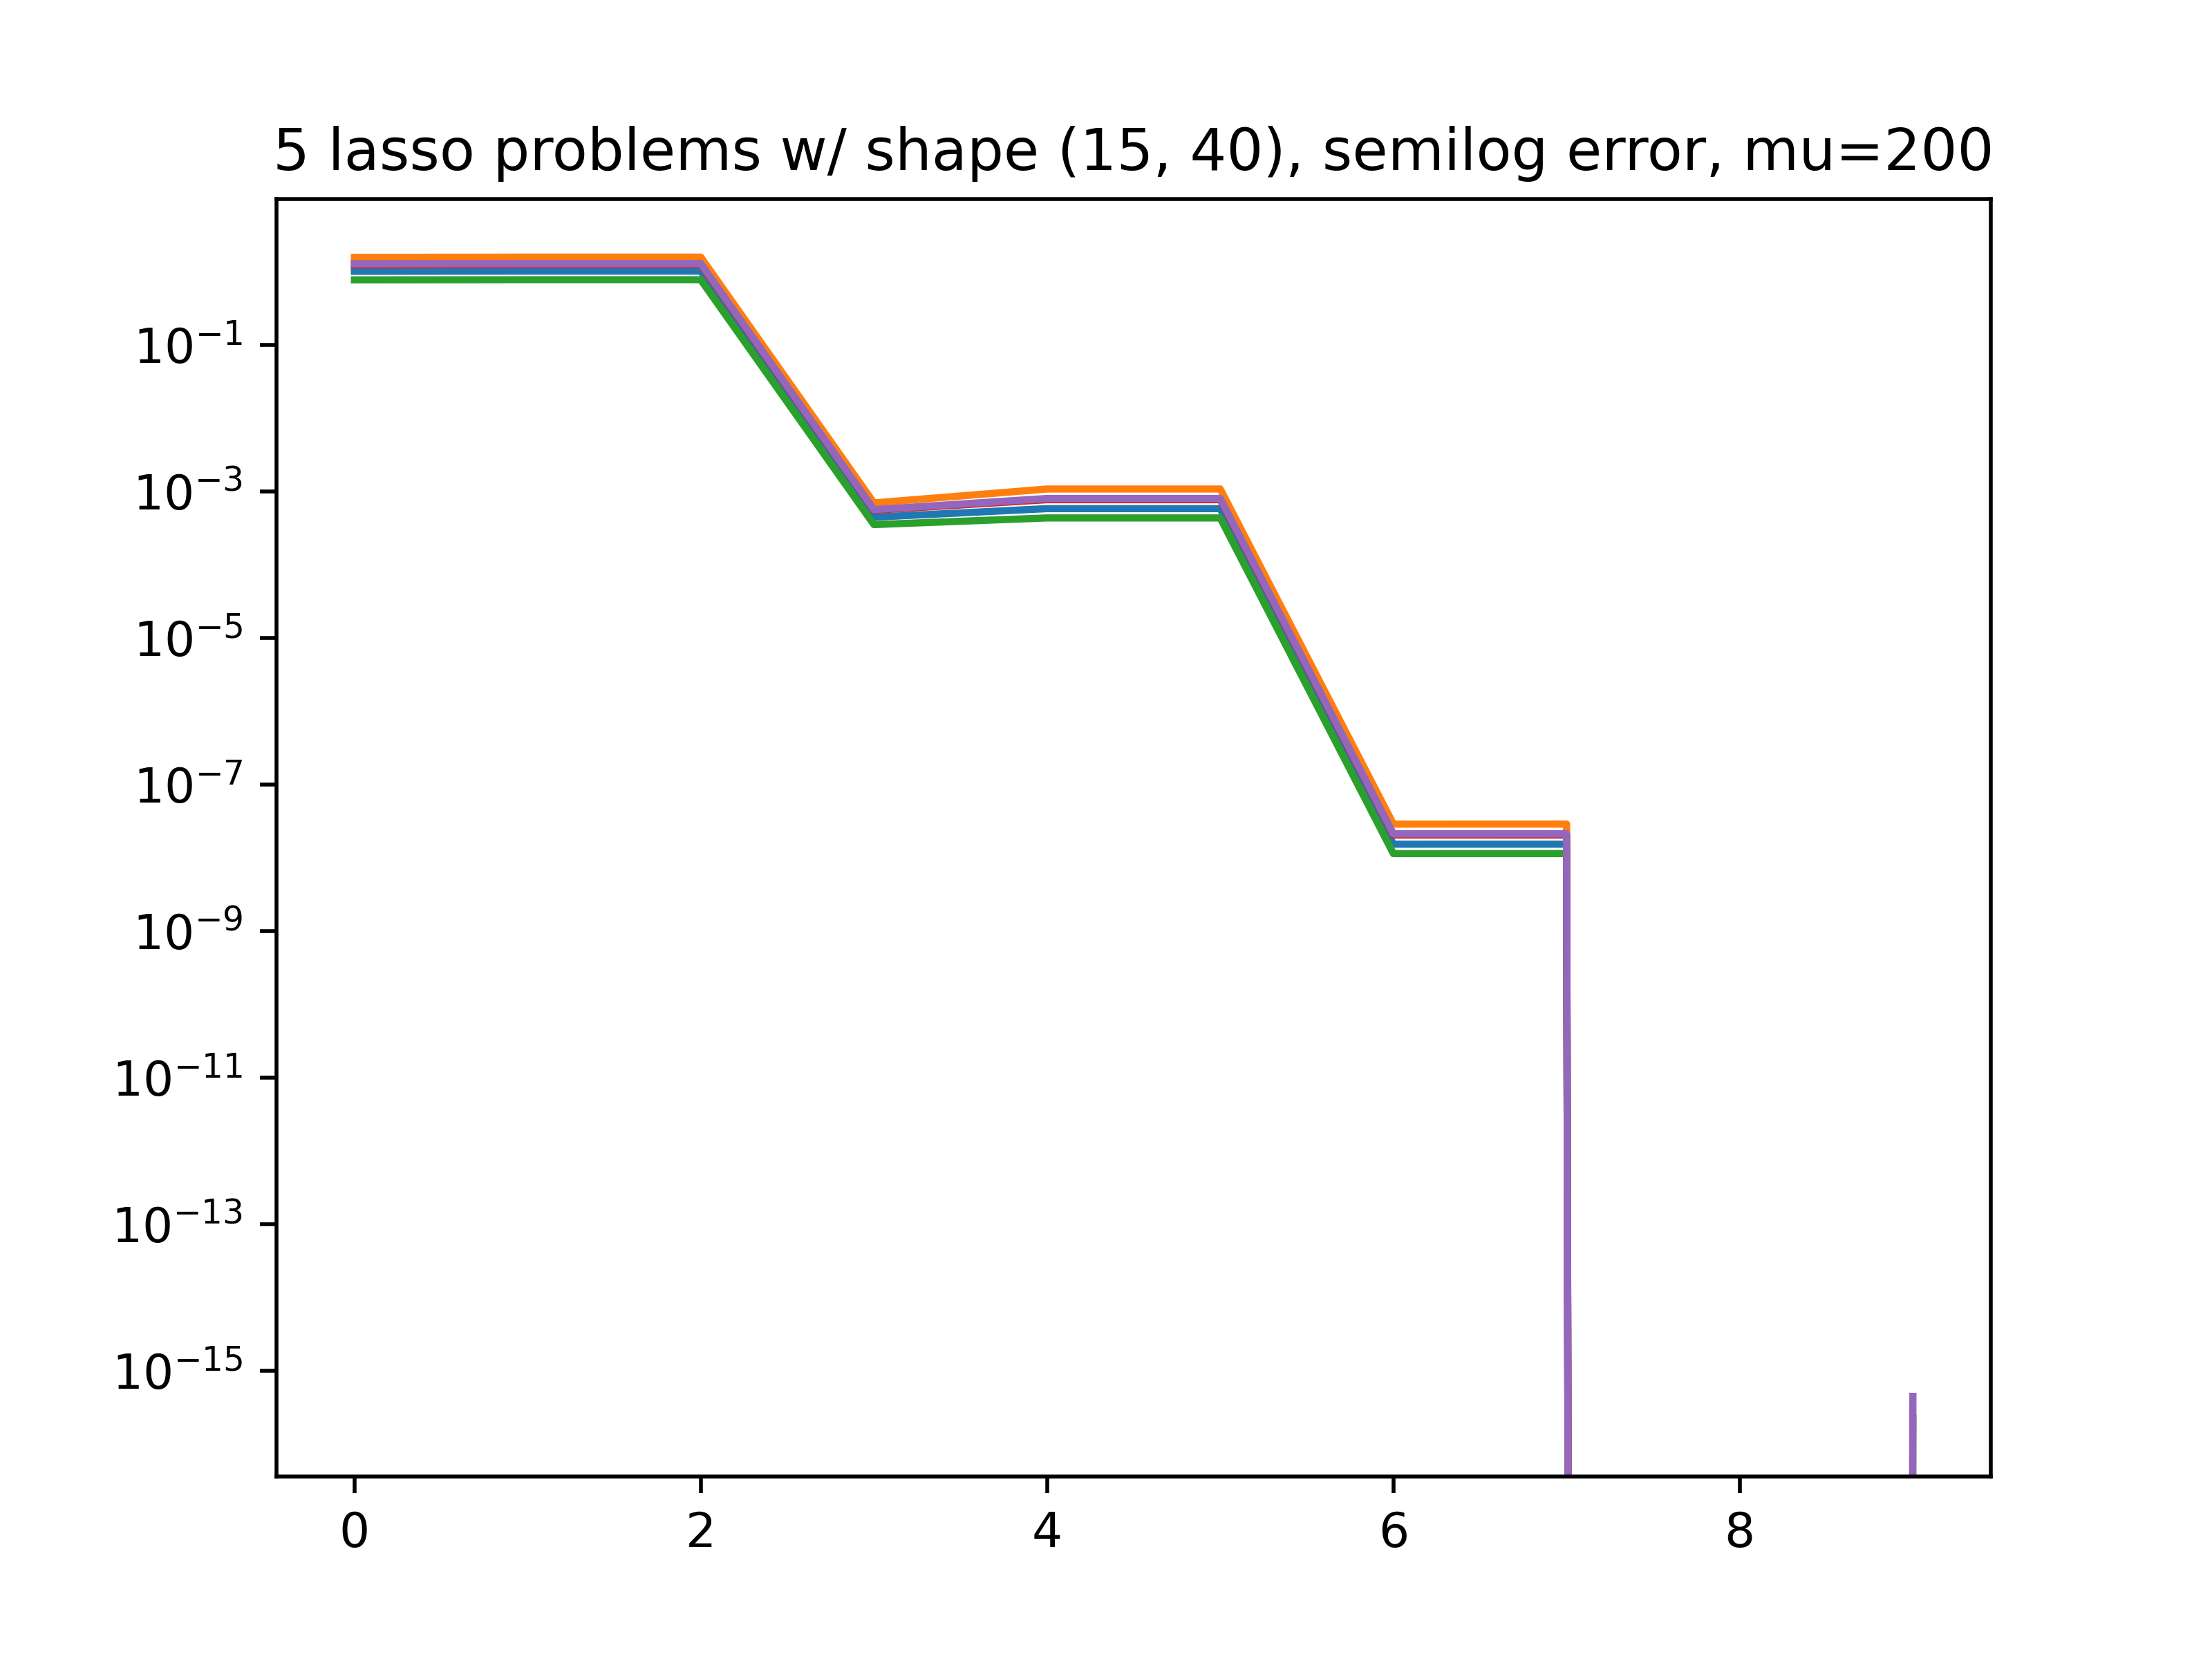
\includegraphics[width=.8\linewidth]{lasso_qp_200.png}
  \caption{1b}
  \label{fig:sfig2}
\end{subfigure}
\caption{Log-scaled error $f(v_t)-f^*$ for $\mu\in \{2, 10, 15, 50, 75, 100, 150, 200$\}.}
\label{fig:fig}
\end{figure}
}
%
\begin{figure}
    \centering
    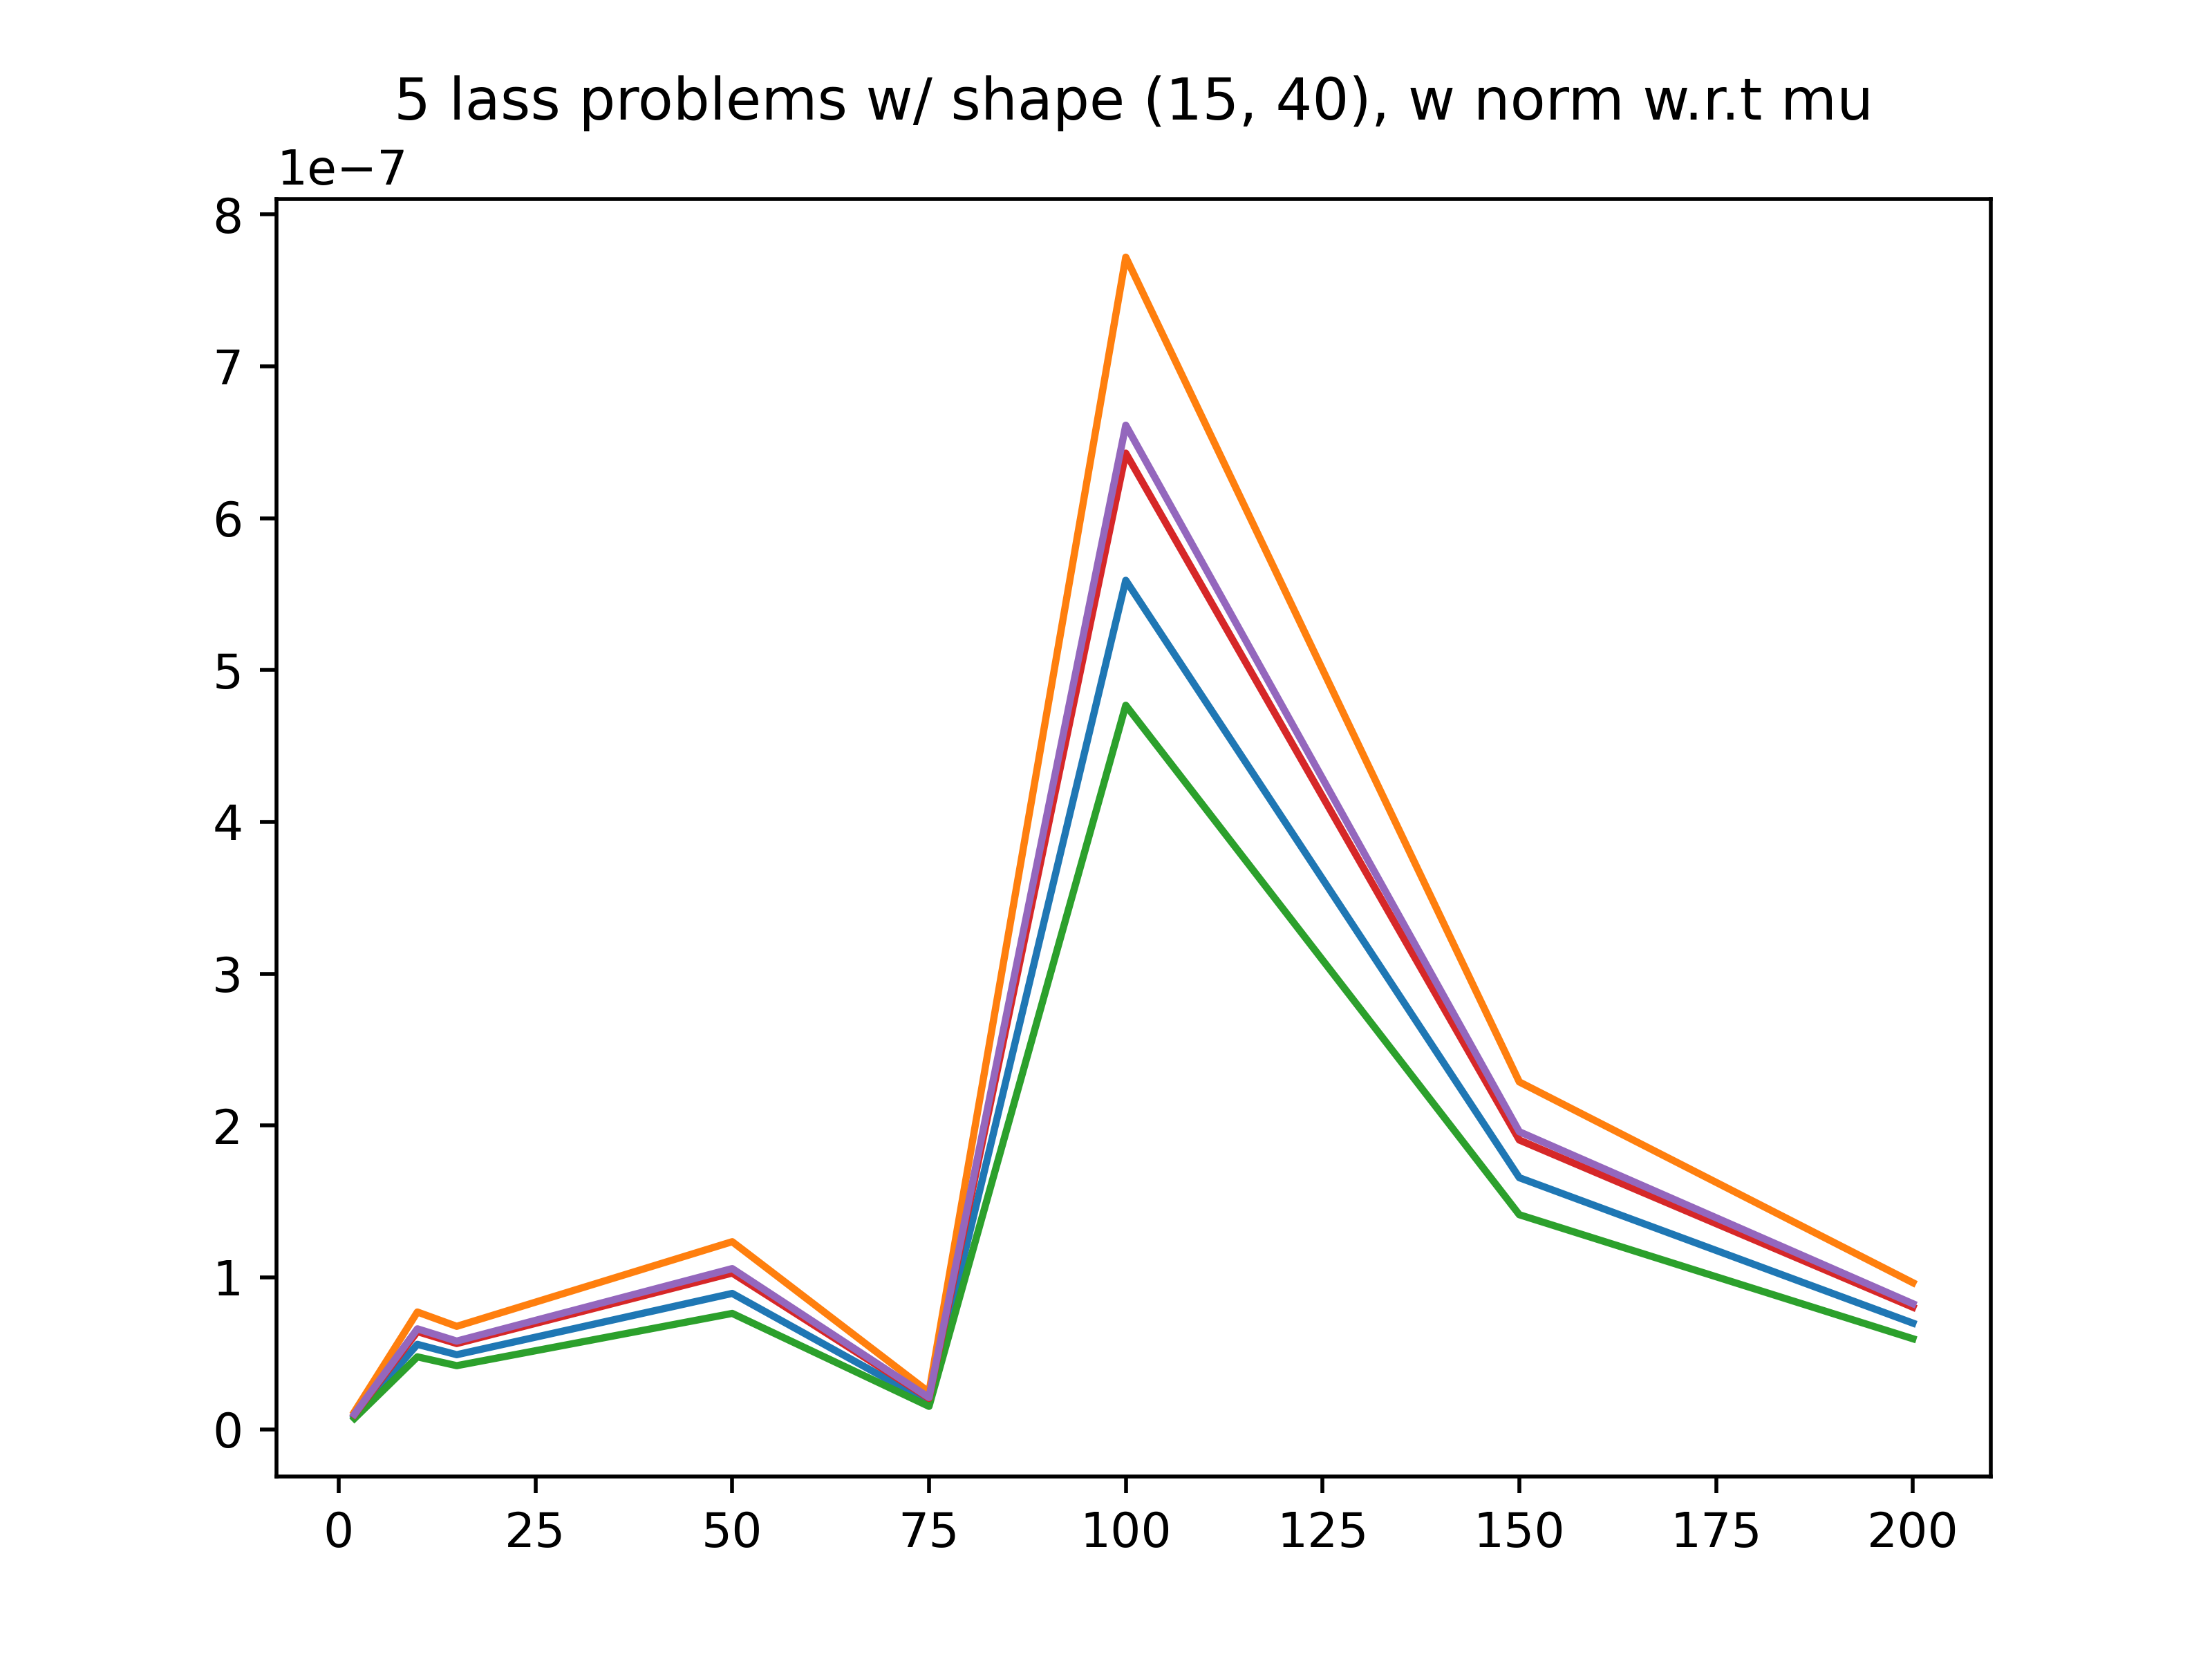
\includegraphics{lass_qp_norm_mus.png}
    \caption{$\norm{w^*}$ w.r.t $\mu$}
    \label{fig:enter-label}
\end{figure}
%
There is a non-trivial relation between $\norm{w}$ and $\mu$. However, one may be interested in doing this plot for different $X$ and $y$ that are not uniformly distributed. Indeed, we expect $w$ to be close to $0$ as there are no expected linear relationship between $X$ and $y$. However, one may be interested in choosing $\mu$ such that $\norm{w}$ is maximized in order for the linear relationship to be as significant as possible. In that case, a proper choice for $\mu$ is approximately $100$.
\newpage 
\textsc{qp.py}
\begin{python}
import jax
import jax.numpy as jnp

jax.config.update('jax_enable_x64', True)
max_iter = 100
max_iter_centering = 10  # ~ ceil(log(m eps) / log(mu)) ~= 10


@jax.jit
def qp(v, Q, p):
    """
    Quadratic program objective function
    """
    return v.T @ Q @ v + p.T @ v


@jax.jit
def centering_step(Q, p, A, b, t, v0, eps, max_iter=max_iter_centering):
    """
    Centering step of the barrier method for quadratic programs:
        min v.T Q v + p.T v
        s.t A v <= b
    Using backtracking line search and Newton's method.
    This code is not optimized for memory usage, there is no need to store all the iterates.
    One can remove vs variable.
    Moreover, since one knows the gradient and hessian for the QP. barrier objective, no need to use jax.grad and jax.hessian.
    """

    def centering_objective(t, v):
        return t * qp(v, Q, p) - jnp.sum(jnp.log(b - A @ v))

    def cond(args):
        n_iter, lambda_square, _, _, _ = args
        return (lambda_square / 2 > eps) & (n_iter < max_iter)

    def iter_newton(inps):
        n_iter, _, v, vs, t = inps
        jac, hessian = jax.grad(centering_objective, argnums=1)(t, v), jax.hessian(centering_objective, argnums=1)(t, v)
        descent_step = - jnp.linalg.solve(hessian, jac)
        lambda_square = - jac.T @ descent_step
        _, t_star = backtracking_line_search(v, descent_step, lambda_square)
        v += t_star * descent_step
        vs = vs.at[n_iter].set(v)
        return n_iter + 1, lambda_square, v, vs, t

    beta = 0.5
    alpha = 0.1

    def backtracking_line_search(v, descent_step, lambda_square, max_iter=10):
        def cond(inps):
            n_iter, t_p = inps
            return ((centering_objective(t, v + t_p * descent_step) >= centering_objective(t,
                                                                                           v) - alpha * t_p * lambda_square) | (
                        jnp.any(A @ (v + t_p * descent_step) >= b)
                    )) & (n_iter < max_iter)

        def iter_backtracking(inps):
            n_iter_bt, t_p = inps
            t_p *= beta
            return n_iter_bt + 1, t_p

        bt = jax.lax.while_loop(cond, iter_backtracking, (0, 1.0))
        return bt

    vs0 = jnp.zeros((max_iter, *v0.shape))
    n_iter, _, v, vs, t = jax.lax.while_loop(cond, iter_newton, (0, 3 * eps, v0, vs0, t))
    return n_iter, v, vs


@jax.jit
def barr_method(Q, p, A, b, v0, eps, mu=10, max_iter=max_iter):
    """
    Barrier method for quadratic programs.
    This code is not optimized for memory usage, there is no need to store all the iterates.
    One can remove vs variable.
    """
    m = b.shape[0]

    def iter_barrier(inps):
        n_iter, n_iters_centering, v, vs, t = inps
        n_iter_centering, v_star, vs_centering = centering_step(Q, p, A, b, t, v,
                                                                eps)  # n_iter_centering must be hardcoded
        n_iters_centering = n_iters_centering.at[n_iter].set(n_iter_centering)
        vs = vs.at[n_iter].set(vs_centering)
        t *= mu
        return n_iter + 1, n_iters_centering, v_star, vs, t

    def cond(args):
        n_iter, _, _, _, t = args
        return (m / t > eps) & (n_iter < max_iter)

    vs0 = jnp.zeros((max_iter, max_iter_centering, *v0.shape))
    vs0 = vs0.at[0].set(jnp.full((max_iter_centering, *v0.shape), v0))
    n_iter, n_iters_centering, v_optimal, vs, _ = jax.lax.while_loop(cond, iter_barrier,
                                                                     (1, jnp.zeros((max_iter, ),
                                                                                  dtype=int), v0, vs0, 1))
    return n_iter, n_iters_centering, v_optimal, vs

\end{python}

\textsc{lasso.py}

\begin{python}
import jax.numpy as jnp
import jax
from qp import barr_method, qp


@jax.jit
def from_dual_to_primal(v, X, y):
    return jnp.linalg.lstsq(X, y + v)[0]


@jax.jit
def lasso_objective(w, X, y, penalization):
    return 1 / 2 * jnp.linalg.norm(X @ w - y) ** 2 + penalization * jnp.linalg.norm(w, ord=1)


@jax.jit
def cast_lasso_to_qp(X, y, penalization):
    n, d = X.shape
    Q = jnp.eye(n) / 2
    p = y
    A = jnp.vstack([X.T, -X.T])
    b = jnp.full(2 * d, penalization)
    return Q, p, A, b


@jax.jit
def solve_lasso(X, y, penalization, mu, eps=1e-16):
    shape = X.shape
    Q, p, A, b = cast_lasso_to_qp(X, y, penalization)
    feasible_v = jnp.zeros((shape[0],))

    n_iter, n_iters_centering, _, duals = barr_method(Q, p, A, b, feasible_v, eps, mu)

    shape = duals.shape
    duals = duals.reshape((-1, shape[-1]))

    dual_objective_vmap = jax.vmap(qp, in_axes=(0, None, None))
    lasso_objective_vmap = jax.vmap(lasso_objective, in_axes=(0, None, None, None))
    from_dual_to_primal_vmap = jax.vmap(from_dual_to_primal, in_axes=(0, None, None))

    primals = from_dual_to_primal_vmap(duals, X, y)
    values_for_dual_objective = dual_objective_vmap(duals, Q, p)
    lasso_objective_values = lasso_objective_vmap(primals, X, y, penalization)

    primals = primals.reshape((*shape[:-1], primals.shape[-1]))
    values_for_dual_objective = values_for_dual_objective.reshape(shape[:-1])
    lasso_objective_values = lasso_objective_values.reshape(shape[:-1])

    return n_iter, n_iters_centering, duals, primals, values_for_dual_objective, lasso_objective_values
\end{python}

\textsc{test.py}
\begin{python}
import jax
import jax.numpy as jnp
from lasso import solve_lasso
from timeit import timeit
import matplotlib.pyplot as plt
import numpy as np

N = 5  # number of lasso problems
OP_key = jax.random.PRNGKey(0)  # seed
keys = jax.random.split(OP_key, N)

shape = (15, 40)
mus = jnp.array([2, 10, 15, 50, 75, 100, 150, 200])
penalization = 10
distrib = jax.random.uniform

wnorm = np.zeros((len(mus), N))  # for storage purpose
las_obj = np.zeros((len(mus), N))

for idx, mu in enumerate(mus):
    @timeit
    @jax.vmap
    def wrapper_lasso_barr_method(key):
        X, y = distrib(key, shape=shape), distrib(key, shape=(shape[0],))
        return solve_lasso(X, y, penalization=penalization, mu=mu, eps=1e-6)


    n_iters, n_iters_centering, _, primals, values_for_dual_objective, lasso_objective_values = wrapper_lasso_barr_method(
        keys)

    for i in range(N):
        iteration = n_iters[i]
        reconstructed_values_for_dual_objective = jnp.concatenate(
            [(values_for_dual_objective[i][:iteration][j][:n_iters_centering[i][j]]) for j in
             range(iteration)])

        min = jnp.min(reconstructed_values_for_dual_objective)
        plt.semilogy(range(len(reconstructed_values_for_dual_objective)), reconstructed_values_for_dual_objective - min)

    plt.title(f"{N} lasso problems w/ shape {shape[0], shape[1]}, semilog error, mu={mu}")
    plt.savefig(f"./plots/lasso_qp_{mu}", dpi=500)
    plt.close()

    for i in range(N):
        iteration = n_iters[i]
        reconstructed_values_for_primal = jnp.linalg.norm(jnp.concatenate(
            [(primals[i][:iteration][j][:n_iters_centering[i][j]]) for j in
             range(1, n_iters[i])]),
            axis=-1)[-1]
        wnorm[idx][i] = reconstructed_values_for_primal[-1]
        plt.semilogy(range(len(reconstructed_values_for_primal)), reconstructed_values_for_primal)

    plt.title(f"{N} lasso problems w/ shape {shape[0], shape[1]}, norm w, mu={mu}")
    plt.savefig(f"./plots/lasso_qp_norm_{mu}", dpi=500)
    plt.close()

    for i in range(N):
        iteration = n_iters[i]
        reconstructed_values_for_lasso_objective_values = jnp.concatenate(
            [(lasso_objective_values[i][:iteration][j][:n_iters_centering[i][j]]) for j in
             range(iteration)])
        las_obj[idx][i] = reconstructed_values_for_lasso_objective_values[-1]
        plt.semilogy(range(len(reconstructed_values_for_lasso_objective_values)),
                     reconstructed_values_for_lasso_objective_values)

    plt.title(f"{N} lasso problems w/ shape {shape[0], shape[1]}, lasso objective, mu={mu}")
    plt.savefig(f"./plots/lasso_qp_lasso_objective_{mu}", dpi=500)
    plt.close()

for i in range(N):
    plt.plot(mus, wnorm[:, i])
plt.title(f"{N} lass problems w/ shape {shape[0], shape[1]}, w norm w.r.t mu")
plt.savefig(f"./plots/lass_qp_norm_mus", dpi=500)
plt.close()

for i in range(N):
    plt.plot(mus, las_obj[:, i])
plt.title(f"{N} lass problems w/ shape {shape[0], shape[1]}, lasso obj. w.r.t mu")
plt.savefig(f"./plots/lass_qp_obj_mus", dpi=500)
plt.close()

\end{python}
\end{document}
